%% main.tex
%% Copyright 2023 TJ-CSCCG
%
% This work may be distributed and/or modified under the
% conditions of the LaTeX Project Public License, either version 1.3
% of this license or (at your option) any later version.
% The latest version of this license is in
%   http://www.latex-project.org/lppl.txt
% and version 1.3 or later is part of all distributions of LaTeX
% version 2003/12/01 or later.
%
% This work has the LPPL maintenance status "maintained".
%
% This Current Maintainer of this work is Rizhong Lin.
%
% This work consists of all the *.tex and *.sty files in
%   https://github.com/TJ-CSCCG/Tongji-Beamer
\documentclass[aspectratio=169]{ctexbeamer}

\usepackage{booktabs}
\usepackage{graphicx}

\usetheme{tongji}

\title[AutoTestDesign for FitnessAI]{AutoTestDesign: AI 驱动测试设计工具}
\subtitle{以 FitnessAI 为目标应用的详细测试设计与验证}
\author[AutoTestDesign Team]{
    2352017 张睿琦 \quad 2252964 张峻搏 \quad 2352495 张竹和 \\
    2353018 钱宝强 \quad 2353117 黄彦炜
}
\institute[Dept.~Comp.~Sci.~\&~Tech., Tongji Univ.]{
    Department of Computer Science and Technology, Tongji University \\
    同济大学计算机科学与技术学院软件工程系
}

\date{2026-05-30}

\begin{document}

\begin{frame}
    \titlepage
\end{frame}

%% introduction.tex
%% Copyright 2023 TJ-CSCCG
%
% This work may be distributed and/or modified under the
% conditions of the LaTeX Project Public License, either version 1.3
% of this license or (at your option) any later version.
% The latest version of this license is in
%   http://www.latex-project.org/lppl.txt
% and version 1.3 or later is part of all distributions of LaTeX
% version 2003/12/01 or later.
%
% This work has the LPPL maintenance status "maintained".
%
% This Current Maintainer of this work is Rizhong Lin.
%
% This work consists of all the *.tex and *.sty files in
%   https://github.com/TJ-CSCCG/Tongji-Beamer
\section{项目背景}

\begin{frame}{项目背景}
    \small
    \begin{block}{项目背景}
        \begin{itemize}
            \item 软件测试设计往往依赖人工从需求中抽取覆盖项、风险点与测试策略，成本高且一致性不足。
            \item FitnessAI 同时包含姿态分析、状态机计数、记录过滤、统计聚合等多类业务逻辑，适合作为测试设计工具的验证对象。
            \item 因此我们实现 AutoTestDesign，将需求分析、风险评估、测试设计与交互审查串成一条完整工作流。
        \end{itemize}
    \end{block}
\end{frame}

\begin{frame}{项目目标}
    \small
    \begin{block}{项目目标}
        \begin{itemize}
            \item 构建一个可运行的 AI 驱动测试设计工具，支持需求结构化、QRA、黑盒/白盒设计与导出。
            \item 使用该工具测试 FitnessAI 项目。
            \item 通过自动化执行、Allure 报告和 JaCoCo 覆盖率验证工具输出的有效性。
        \end{itemize}
    \end{block}

    \begin{block}{整体方案}
        \begin{itemize}
            \item 工具：AutoTestDesign（Vue 3 + Express + FastAPI + PostgreSQL）
            \item 目标应用：FitnessAI 智能健身辅助系统
            \item 验证路径：QRA 风险分析 -> 测试计划 -> 详细测试设计 -> 自动化执行与覆盖率证据
        \end{itemize}
    \end{block}
\end{frame}

\begin{frame}{项目范围与产出}
    \begin{columns}[T]
        \column{0.42\textwidth}
        \footnotesize
        \begin{itemize}
            \item 目标接口：
            \item \texttt{/api/analytics/pose}
            \item \texttt{/api/user/\{id\}/records}
            \item \texttt{/api/user/\{id\}/dashboard}
            \item 扩展范围：记录筛选、\texttt{/api/exercises}、reset 接口
            \item 工具输出：10 条结构化需求、10 条风险项、37 个覆盖项、81 条测试用例、6 种设计方法
            \item 验证证据：Markdown / JSON / CSV / Excel + JUnit 5 + Allure + JaCoCo
        \end{itemize}

        \column{0.54\textwidth}
        \begin{figure}
            \centering
            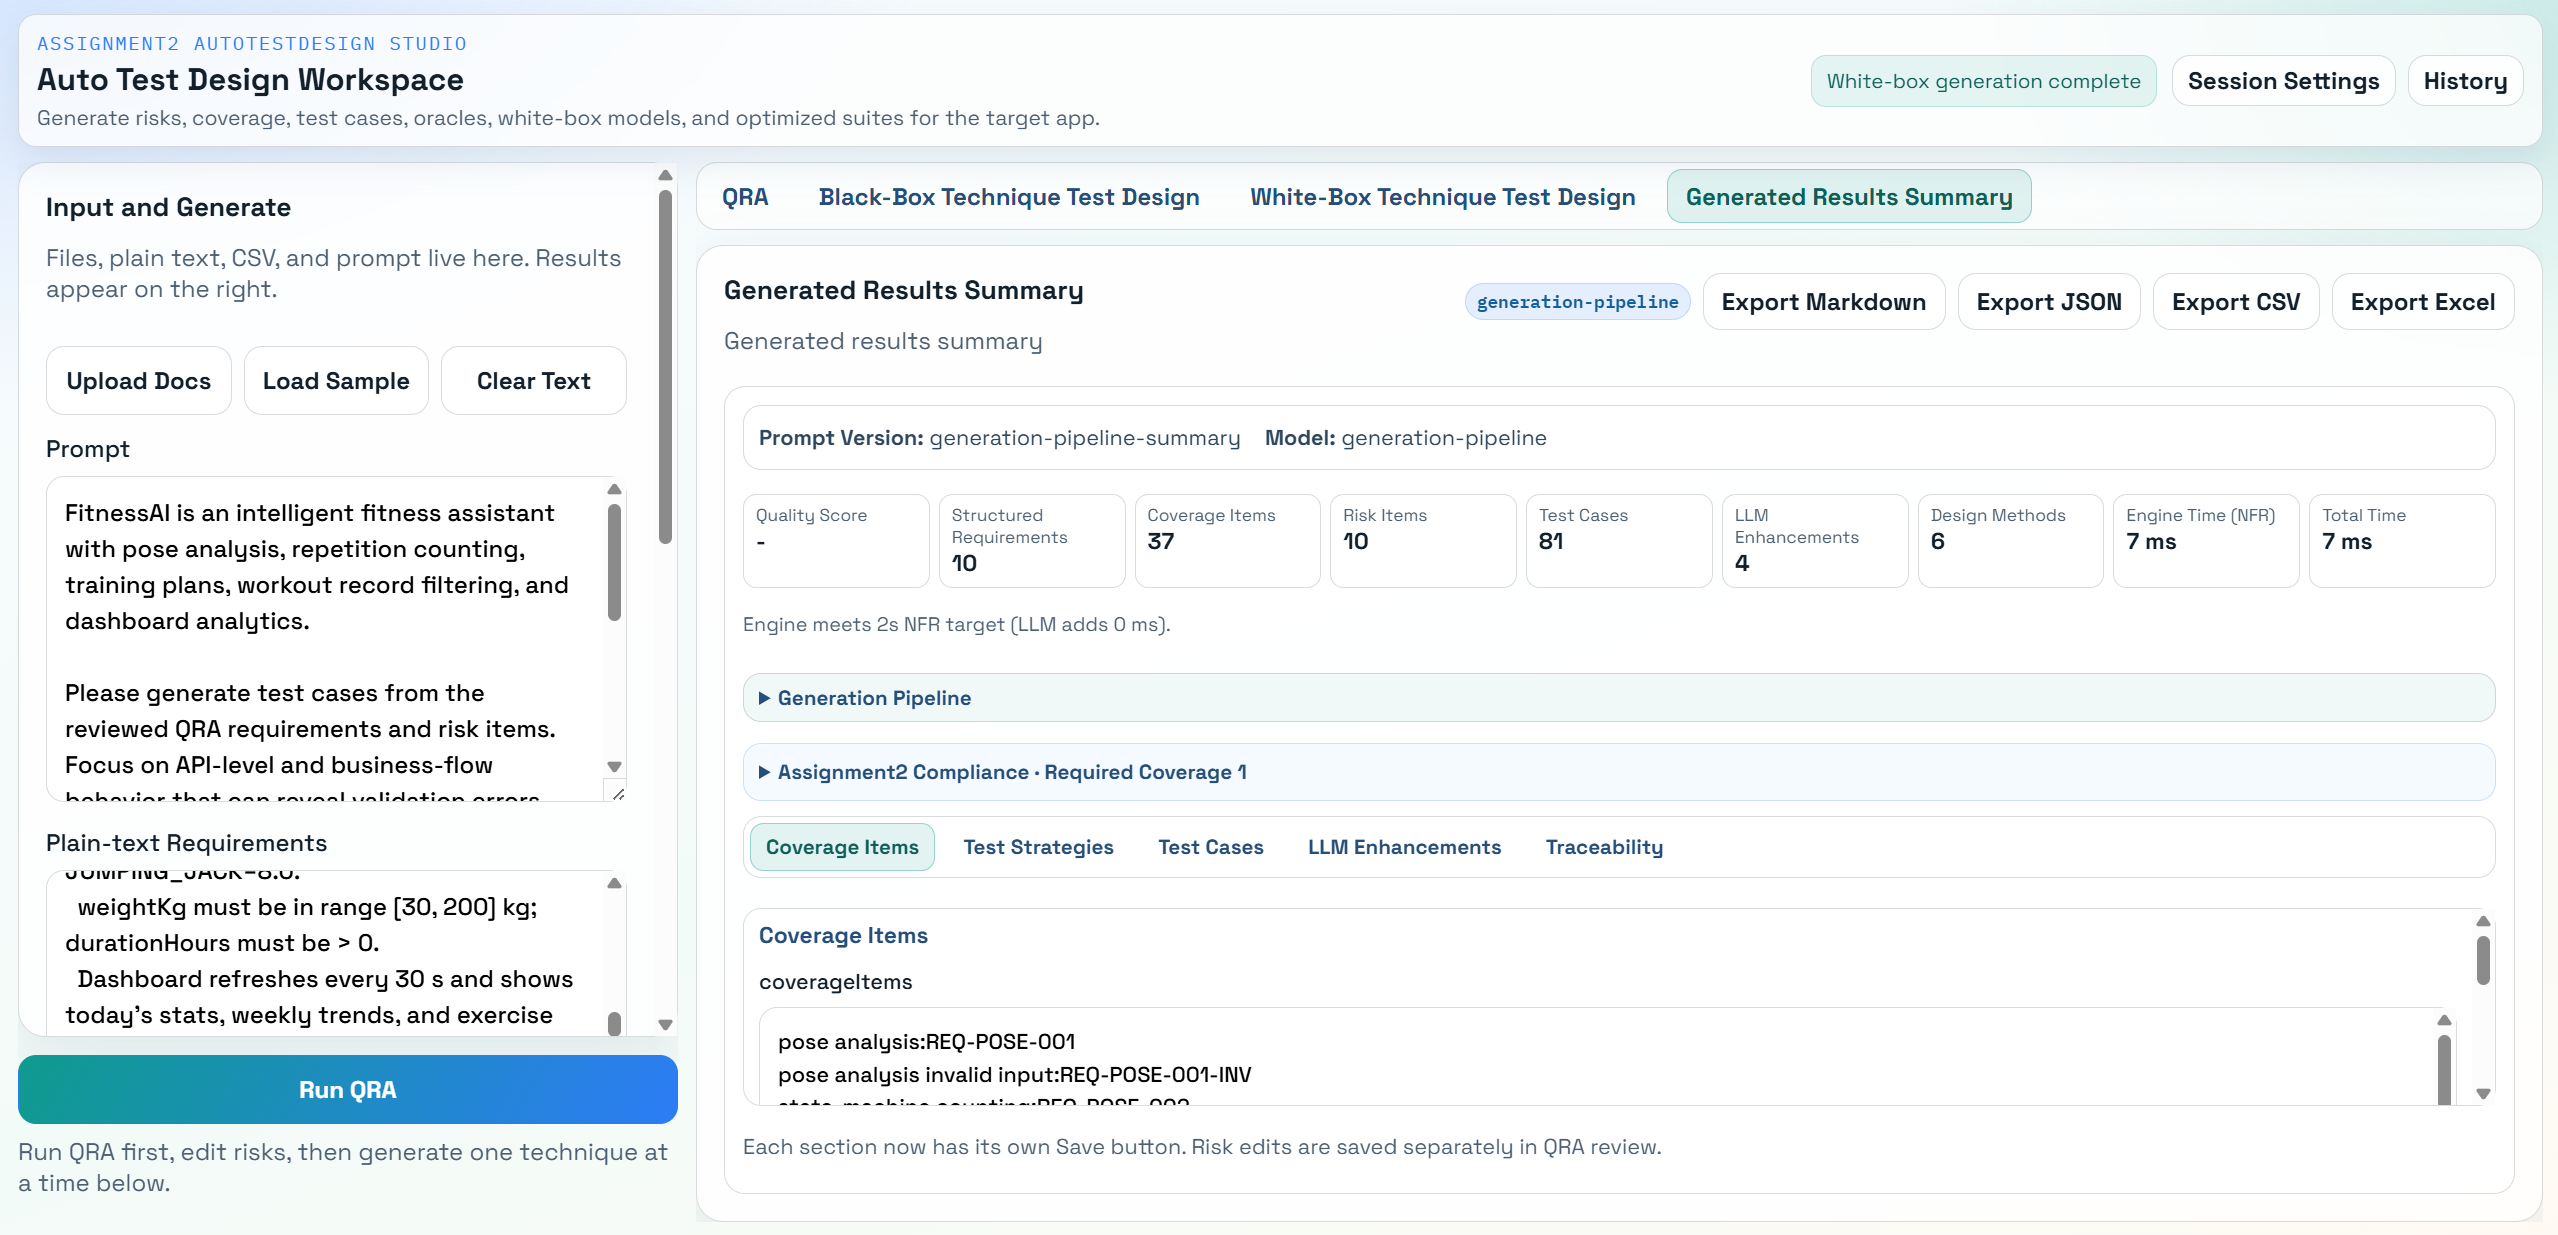
\includegraphics[width=0.98\textwidth]{contents/figure/fitnessai/Summary.png}
        \end{figure}
    \end{columns}
\end{frame}

%% body.tex
%% Copyright 2023 TJ-CSCCG
%
% This work may be distributed and/or modified under the
% conditions of the LaTeX Project Public License, either version 1.3
% of this license or (at your option) any later version.
% The latest version of this license is in
%   http://www.latex-project.org/lppl.txt
% and version 1.3 or later is part of all distributions of LaTeX
% version 2003/12/01 or later.
%
% This work has the LPPL maintenance status "maintained".
%
% This Current Maintainer of this work is Rizhong Lin.
%
% This work consists of all the *.tex and *.sty files in
%   https://github.com/TJ-CSCCG/Tongji-Beamer
\section{Project Analysis}

\begin{frame}{Risk Analysis Evidence}
    \begin{columns}[T]
        \column{0.48\textwidth}
        \begin{figure}
            \centering
            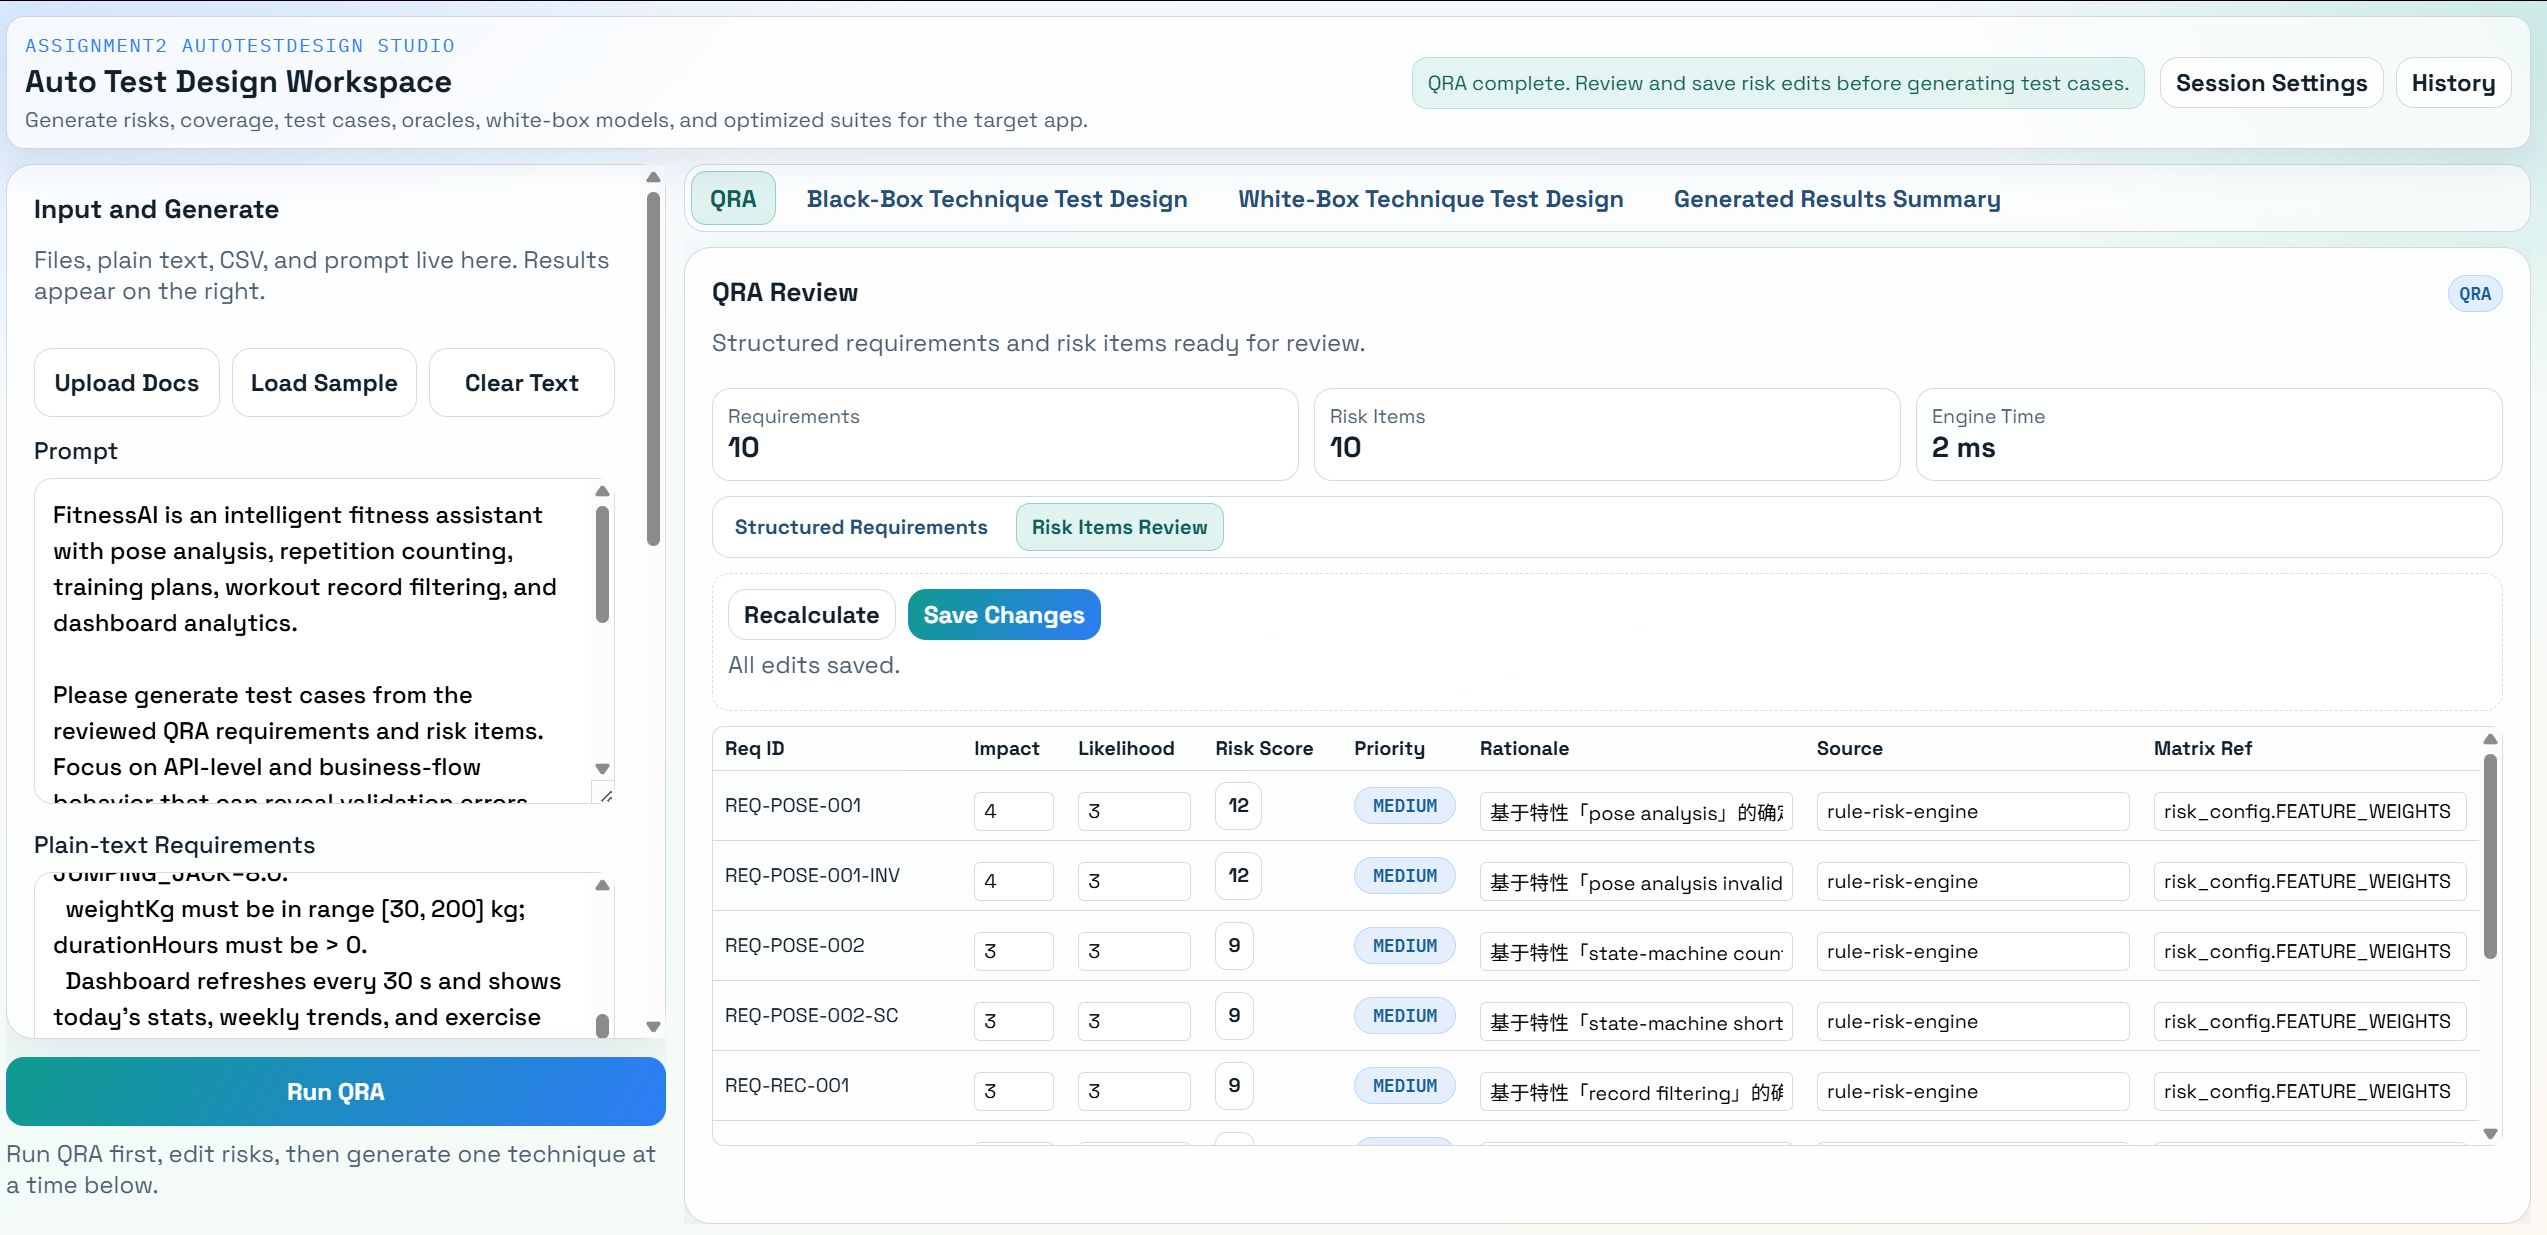
\includegraphics[width=\textwidth]{contents/figure/fitnessai/QRA_1.png}
        \end{figure}

        \column{0.48\textwidth}
        \begin{figure}
            \centering
            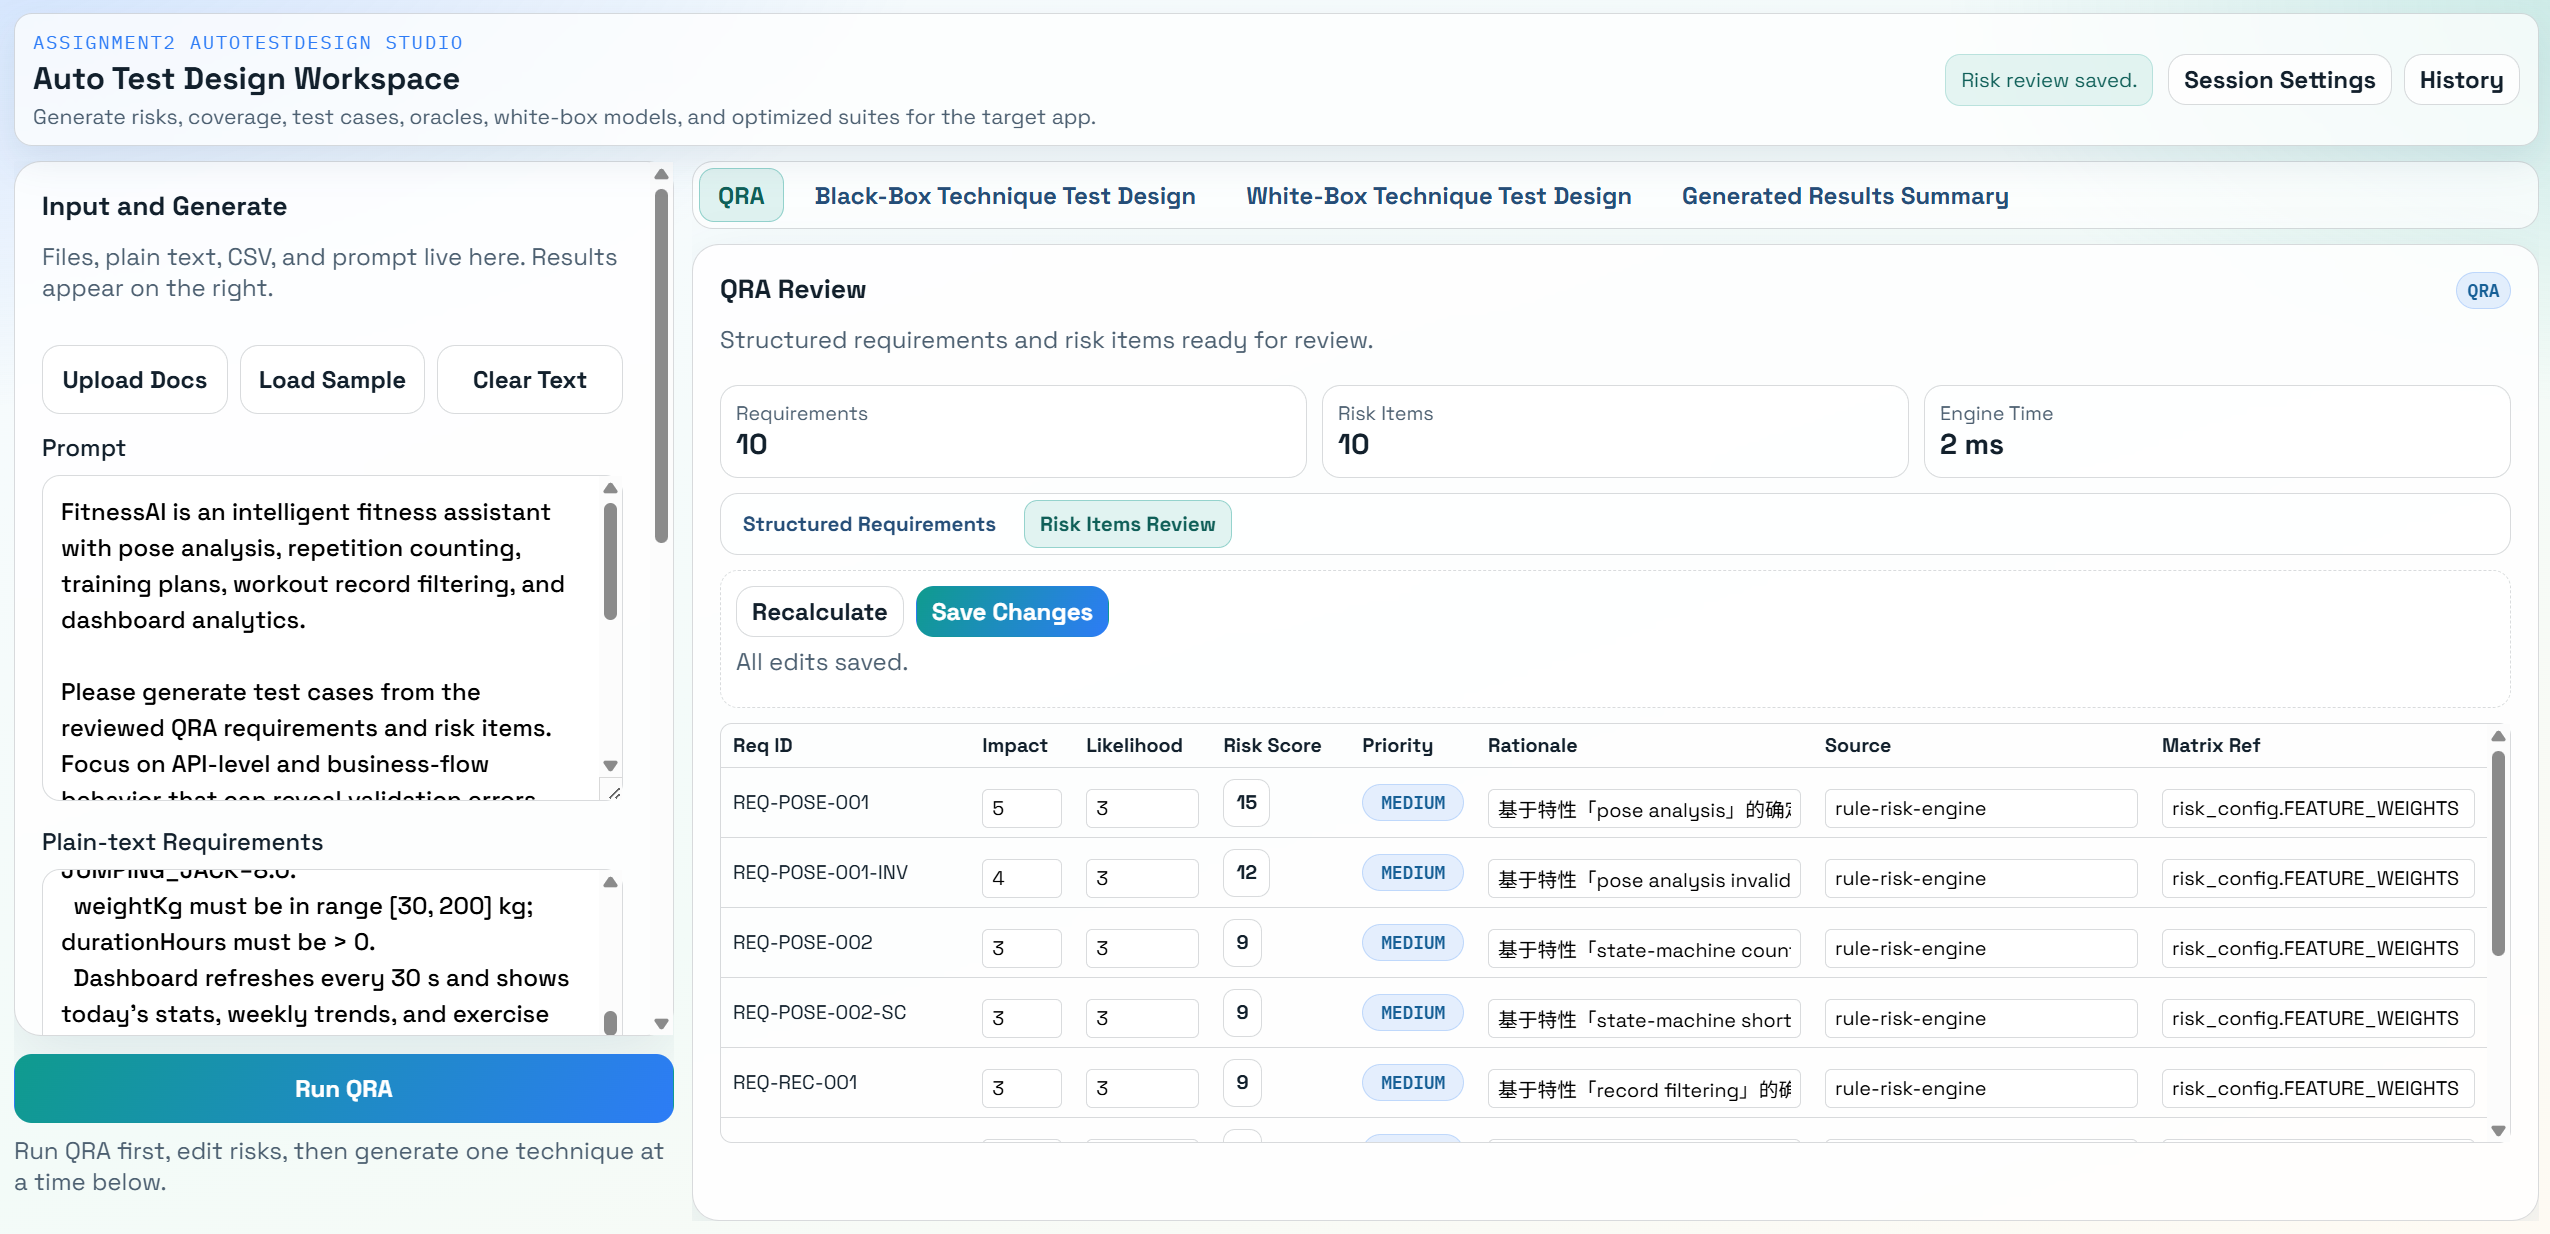
\includegraphics[width=\textwidth]{contents/figure/fitnessai/QRA_change.png}
        \end{figure}
    \end{columns}

    \vspace{0.35em}
    \footnotesize
    \begin{itemize}
        \item The QRA engine generated 10 structured risk items from the FitnessAI requirements
        \item \texttt{REQ-POSE-001} was reviewed from \texttt{Impact = 4} to \texttt{Impact = 5}, so the score changed from \texttt{12} to \texttt{15}
        \item The screenshots show both the initial output and the saved review result
    \end{itemize}
\end{frame}

\begin{frame}{Risk Analysis Findings}
    \small
    \begin{block}{Final Risk Summary}
        \begin{itemize}
            \item The final report contains 22 risks: 10 tool-generated items and 12 reviewer-supplemented items
            \item The most critical risks are unauthorized access, open CORS, high-frequency pose requests, and inconsistent dashboard semantics
            \item These findings directly determine the priority of the later test suites
        \end{itemize}
    \end{block}
\end{frame}

\begin{frame}{Risk-Driven Test Strategy}
    \small
    \begin{block}{High-Priority Risks}
        \begin{itemize}
            \item Unauthorized access on user-related endpoints
            \item Open CORS configuration with \texttt{origins="*"}
            \item High-frequency pose requests in real-time scenarios
            \item Dashboard \texttt{duration} semantics and aggregation consistency
        \end{itemize}
    \end{block}

    \begin{block}{Strategy}
        \begin{itemize}
            \item QRA identifies the highest-risk paths first
            \item Black-box, white-box, and automation effort is then assigned to those paths
        \end{itemize}
    \end{block}
\end{frame}

\begin{frame}{Risk Priority Mapping}
    \begin{columns}[T]
        \column{0.5\textwidth}
        \footnotesize
        \begin{block}{Priority to Suite Mapping}
            \begin{tabular}{@{}ll@{}}
                \toprule
                \textbf{Priority} & \textbf{Target Suite} \\ \midrule
                P1 & Security \\
                P2 & Pose EP/BVA/ST \\
                P3 & Record DT/WBJ \\
                P4 & Dashboard / history \\
                P5 & Regression \\
                \bottomrule
            \end{tabular}
        \end{block}

        \column{0.46\textwidth}
        \footnotesize
        \begin{block}{Why This Order}
            \begin{itemize}
                \setlength{\itemsep}{0.2em}
                \item P1 targets direct security exposure
                \item P2--P3 target core business behavior
                \item P4--P5 cover consistency and regression
            \end{itemize}
            \begin{itemize}
                \setlength{\itemsep}{0.2em}
                \item Fix severe failures first
                \item Then verify high-frequency paths
                \item Finally expand regression coverage
            \end{itemize}
        \end{block}
    \end{columns}
\end{frame}

\begin{frame}{Test Plan Scope}
    \small
    \begin{block}{Test Scope}
        \begin{itemize}
            \item Pose analysis, analyzer reset, record persistence, and history queries
            \item Dashboard aggregation and response-field validation for \texttt{/api/exercises}
            \item Security-risk validation and high-frequency request checks
        \end{itemize}
    \end{block}

    \begin{block}{Planning Principles}
        \begin{itemize}
            \item Risk-first prioritization
            \item Six design techniques integrated in one workflow
            \item Tool generation, review, and execution kept traceable
        \end{itemize}
    \end{block}
\end{frame}

\begin{frame}{Test Plan Inventory}
    \begin{columns}[T]
        \column{0.52\textwidth}
        \footnotesize
        \begin{block}{Test Suites}
            \begin{itemize}
                \item EP: 20 cases
                \item BVA: 30 cases
                \item Decision Table: 16 cases
                \item Pairwise: 6 cases
                \item State Transition: 5 cases
                \item WhiteBox: 4 cases
                \item Total: 81 cases
            \end{itemize}
        \end{block}

        \column{0.42\textwidth}
        \scriptsize
        \begin{tabular}{@{}lc@{}}
            \toprule
            \textbf{Plan Item} & \textbf{Result} \\ \midrule
            Framework & JUnit 5 + MockMvc \\
            Coverage & Risk-first + 6 techniques \\
            Stages & Generation / review / execution \\
            Extensions & Security / performance depth \\
            Cost & 39h vs 70h \\
            Gain & 44\% \\
            \bottomrule
        \end{tabular}
    \end{columns}
\end{frame}

\begin{frame}{Organization}
    \small
    \begin{block}{Team Responsibilities}
        \begin{itemize}
            \item Test design engineer: generates cases with AutoTestDesign and performs interactive review
            \item Test execution engineer: implements 81 cases with JUnit 5 + MockMvc
            \item Development support engineer: prepares the environment, reproduces issues, and confirms fixes
        \end{itemize}
    \end{block}
\end{frame}

\begin{frame}{Workflow}
    \small
    \begin{block}{Closed Loop from Planning to Execution}
        \begin{itemize}
            \item W1: QRA, generation with six techniques, risk review, and artifact export
            \item W2--W3: script implementation and execution of all 81 tests
            \item W3--W4: security / performance supplements and report consolidation
        \end{itemize}
    \end{block}
\end{frame}

\begin{frame}{Detailed Test Design: EP}
    \begin{columns}[T]
        \column{0.42\textwidth}
        \scriptsize
        \begin{block}{Technique}
            \begin{itemize}
                \item EP covers valid and invalid poses, empty requests, record filtering, exercise lists, and dashboard flows
            \end{itemize}
        \end{block}

        \begin{block}{Result}
            \begin{itemize}
                \item EP contributes 20 cases and partitions the core input domain
                \item It gives the first broad black-box coverage layer
            \end{itemize}
        \end{block}

        \column{0.52\textwidth}
        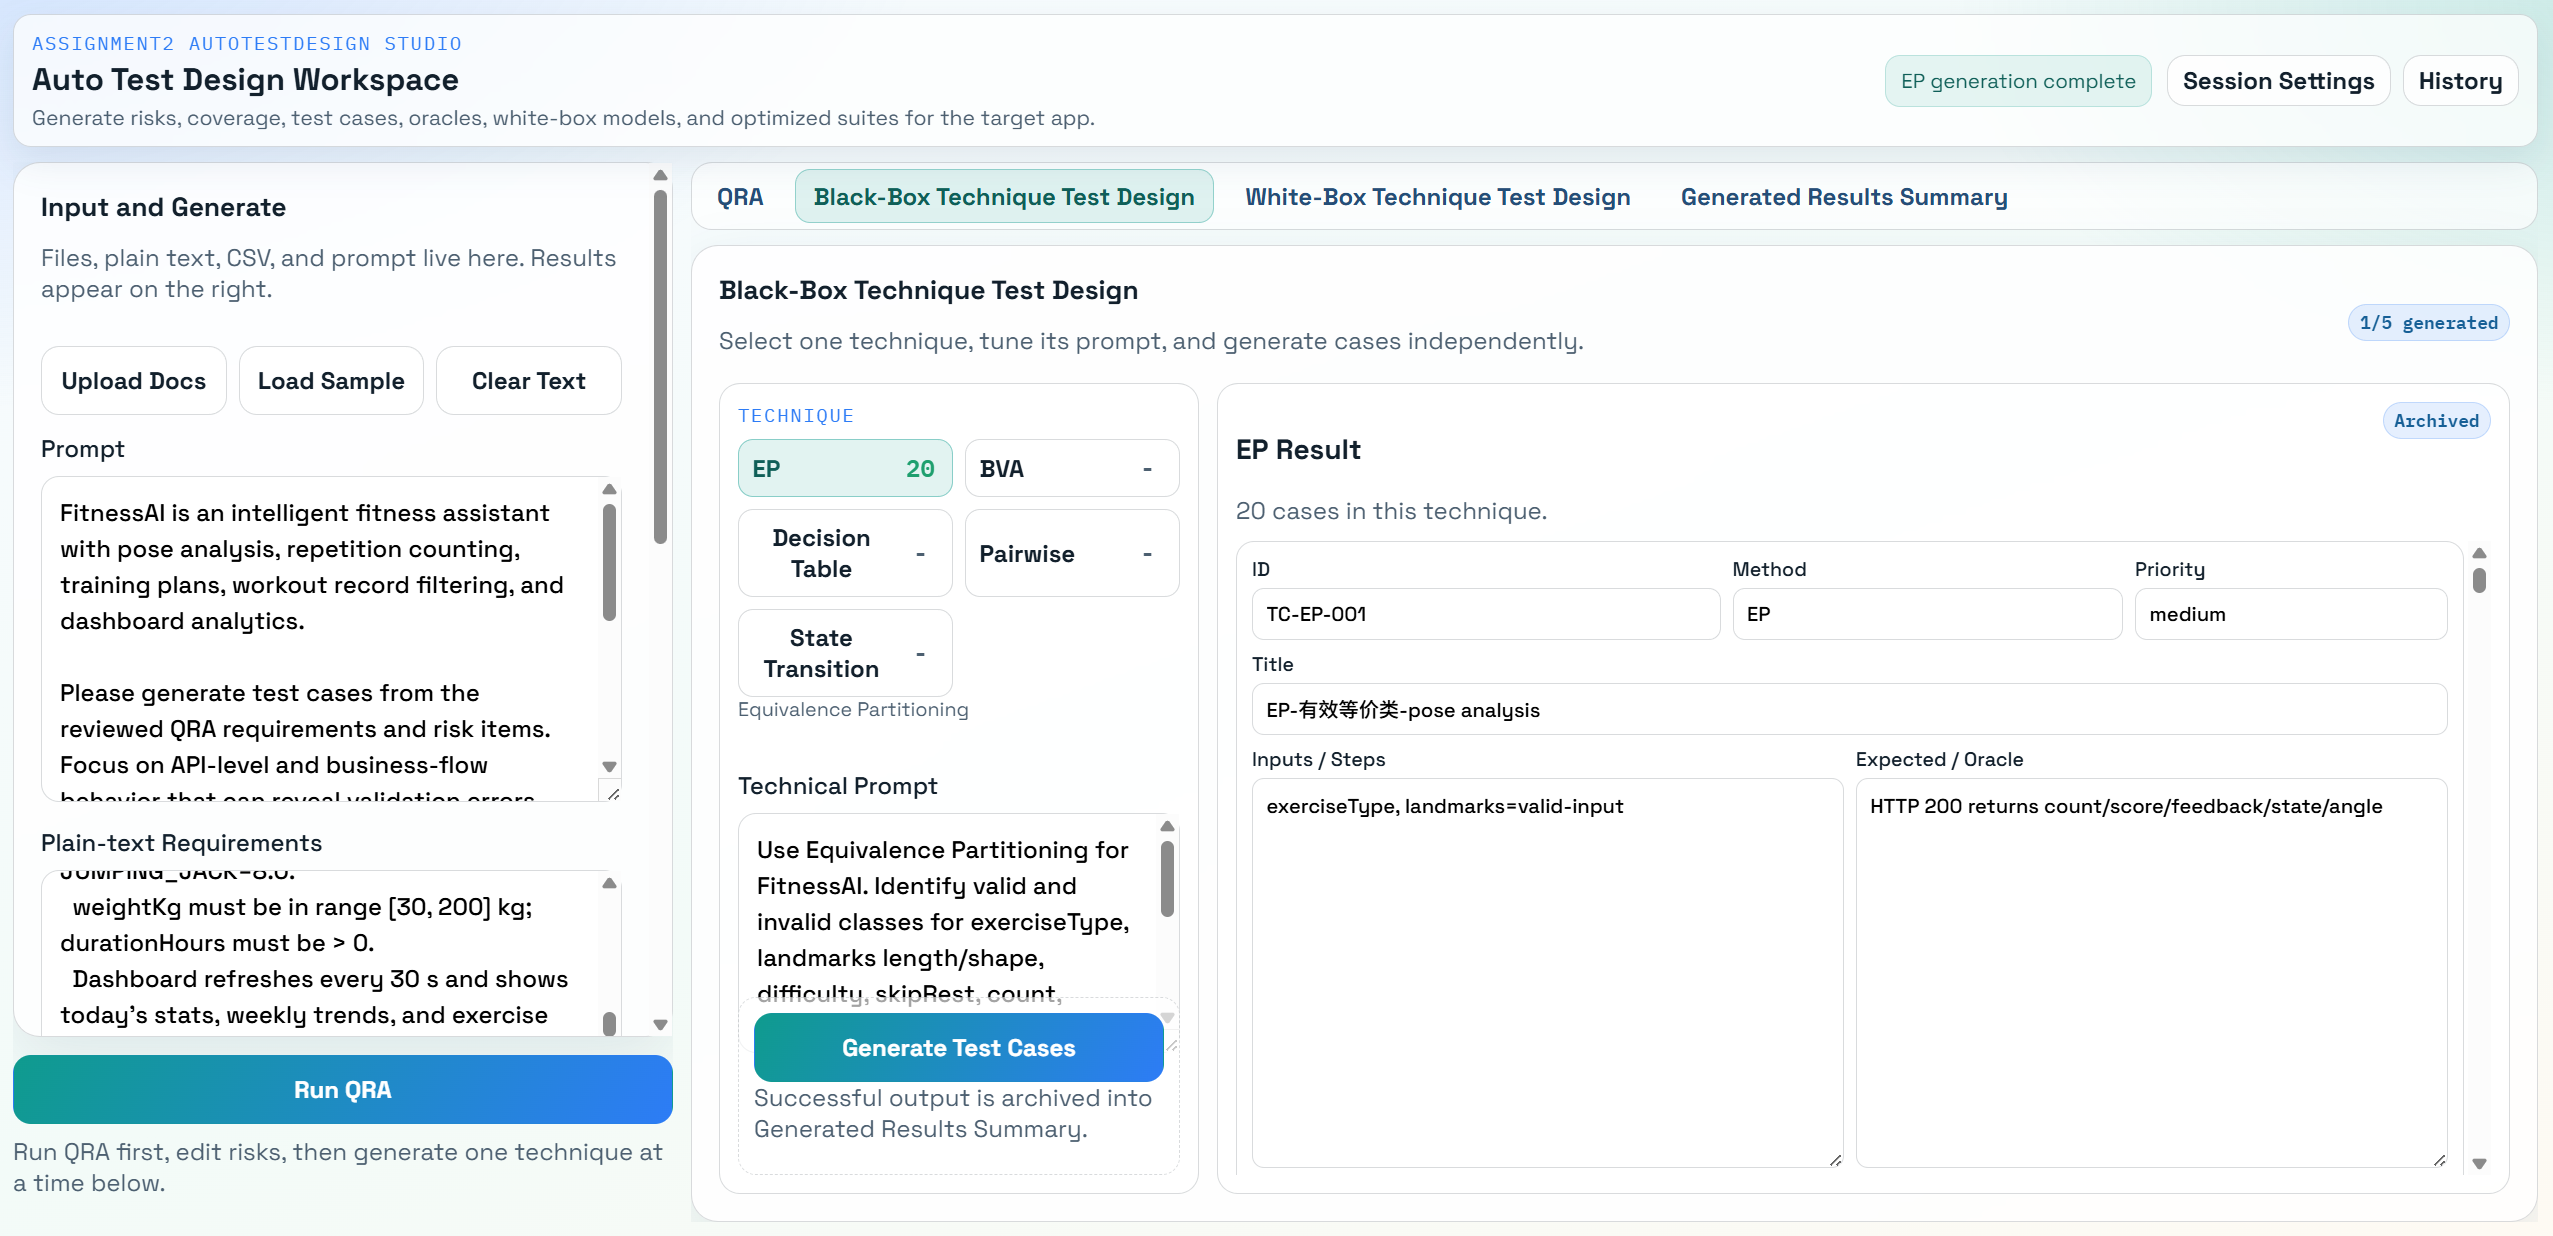
\includegraphics[width=0.9\textwidth]{contents/figure/fitnessai/Black_EP.png}
    \end{columns}
\end{frame}

\begin{frame}{Detailed Test Design: BVA}
    \begin{columns}[T]
        \column{0.42\textwidth}
        \scriptsize
        \begin{block}{Technique}
            \begin{itemize}
                \item BVA covers \texttt{landmarks.length}, \texttt{count}, and \texttt{duration}
            \end{itemize}
        \end{block}

        \begin{block}{Result}
            \begin{itemize}
                \item BVA contributes 30 cases and samples critical boundaries
                \item It is used to verify the risk-sensitive edges of pose and record inputs
            \end{itemize}
        \end{block}

        \column{0.52\textwidth}
        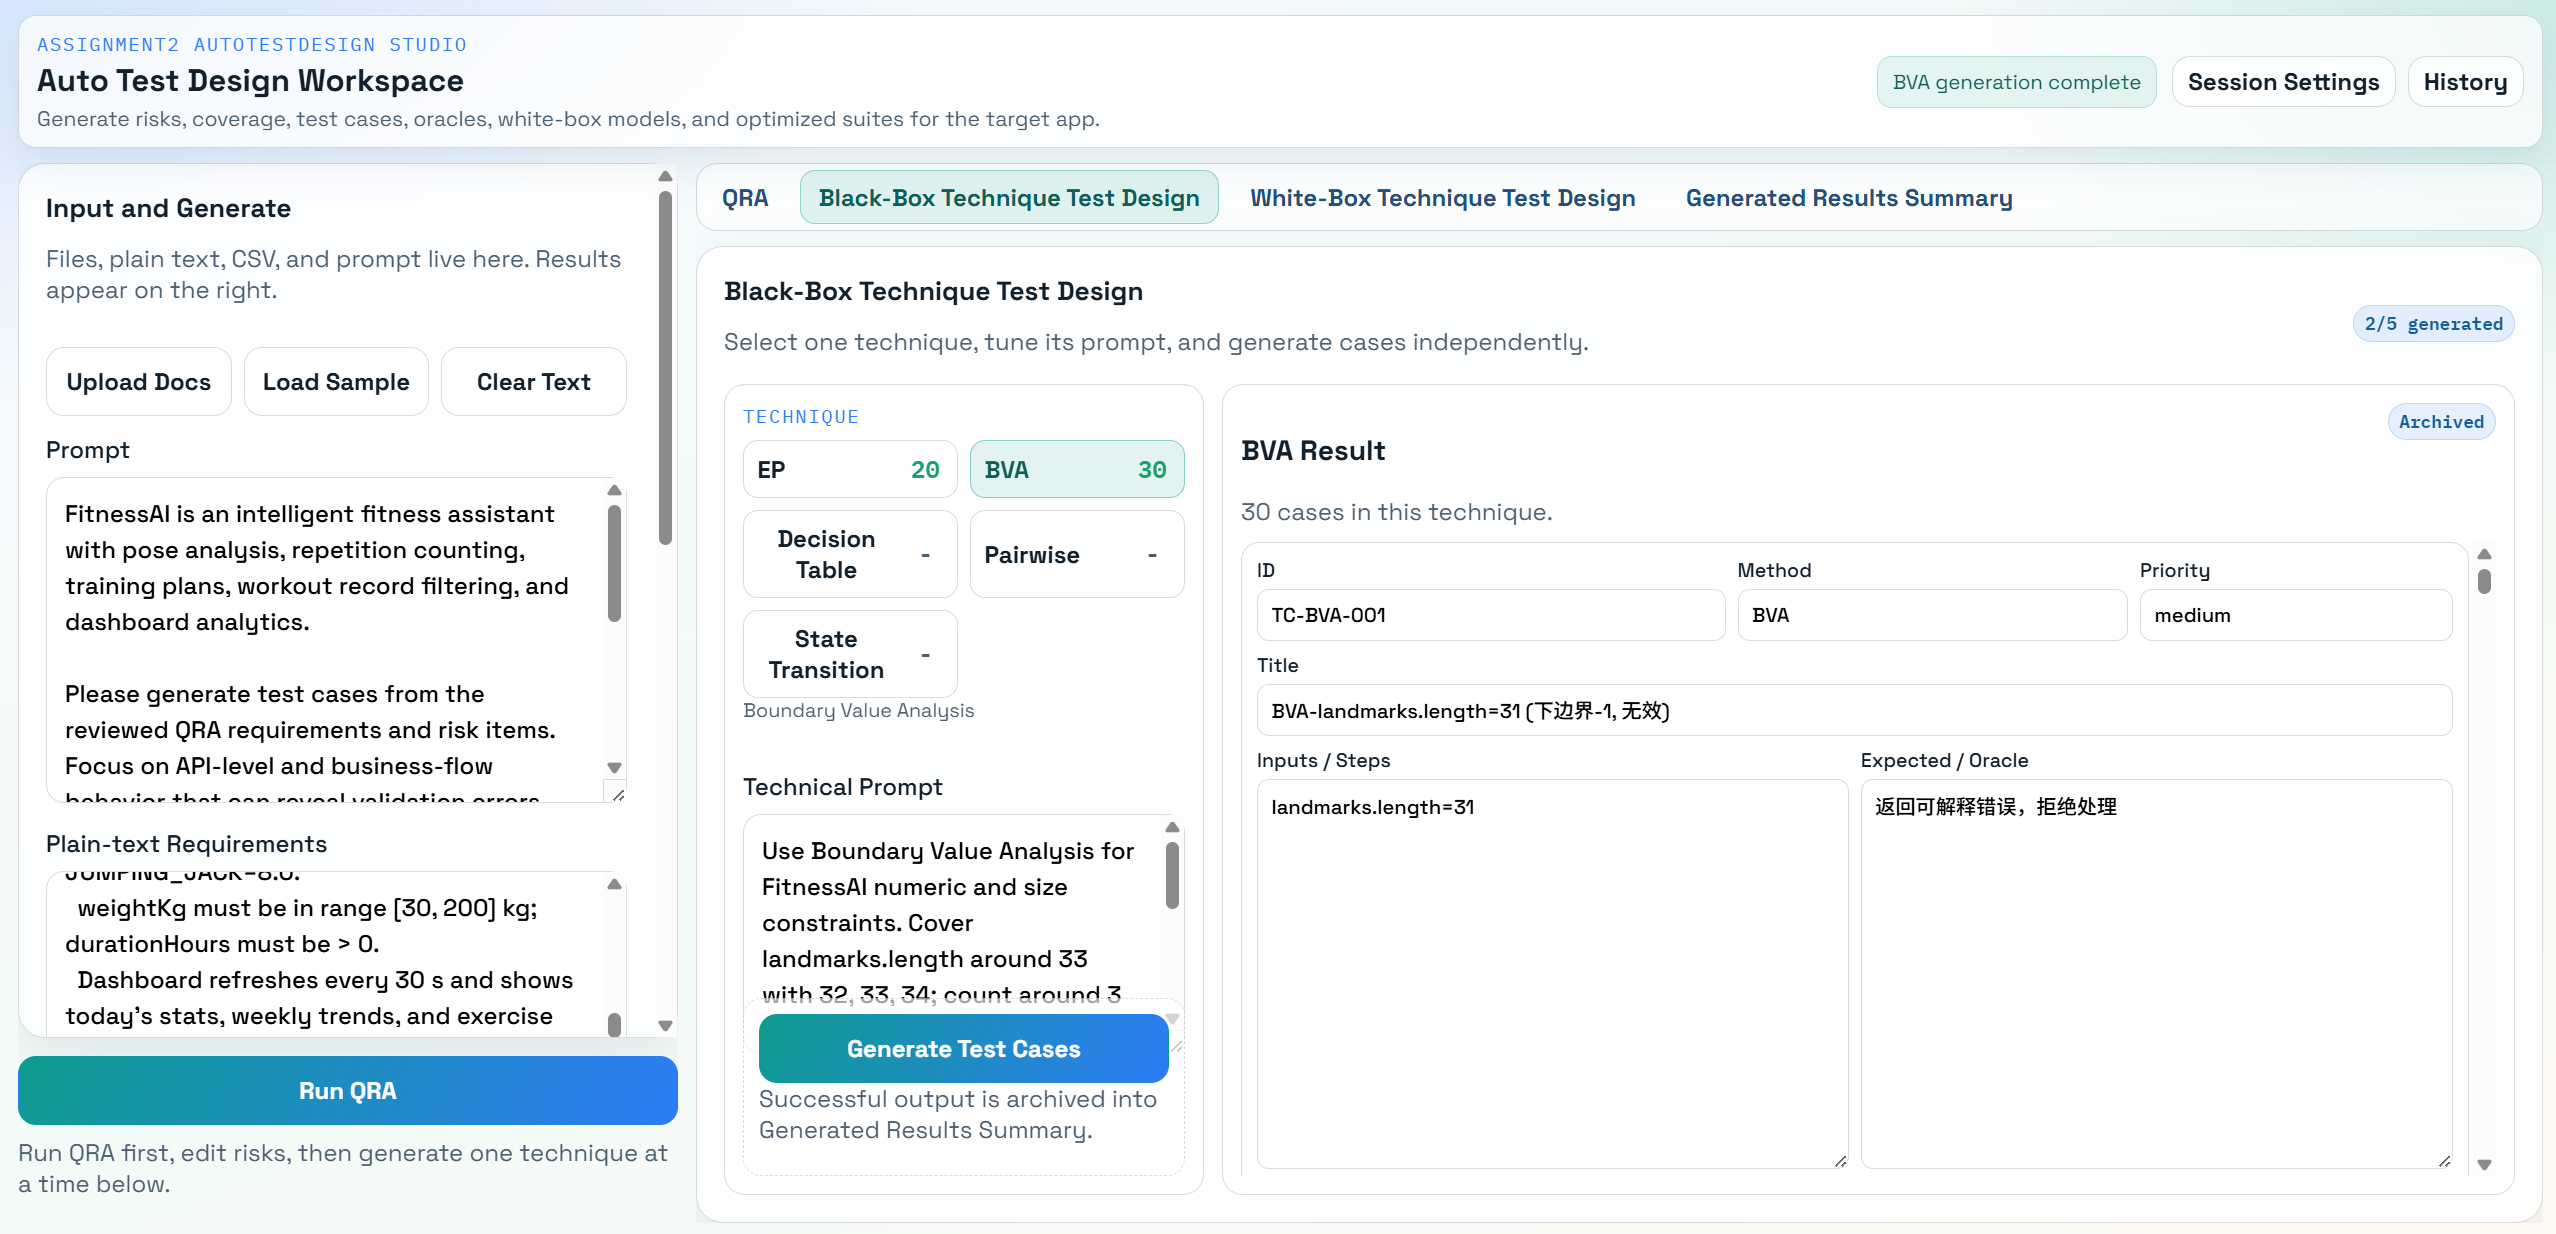
\includegraphics[width=0.9\textwidth]{contents/figure/fitnessai/Black_BVA.png}
    \end{columns}
\end{frame}

\begin{frame}{Detailed Test Design: Decision Table}
    \begin{columns}[T]
        \column{0.42\textwidth}
        \scriptsize
        \begin{block}{Technique}
            \begin{itemize}
                \item Decision Table covers the four record-filtering rules and exercise-list difficulty validation
            \end{itemize}
        \end{block}

        \begin{block}{Result}
            \begin{itemize}
                \item It contributes 16 cases and covers rule combinations directly
            \end{itemize}
        \end{block}

        \column{0.52\textwidth}
        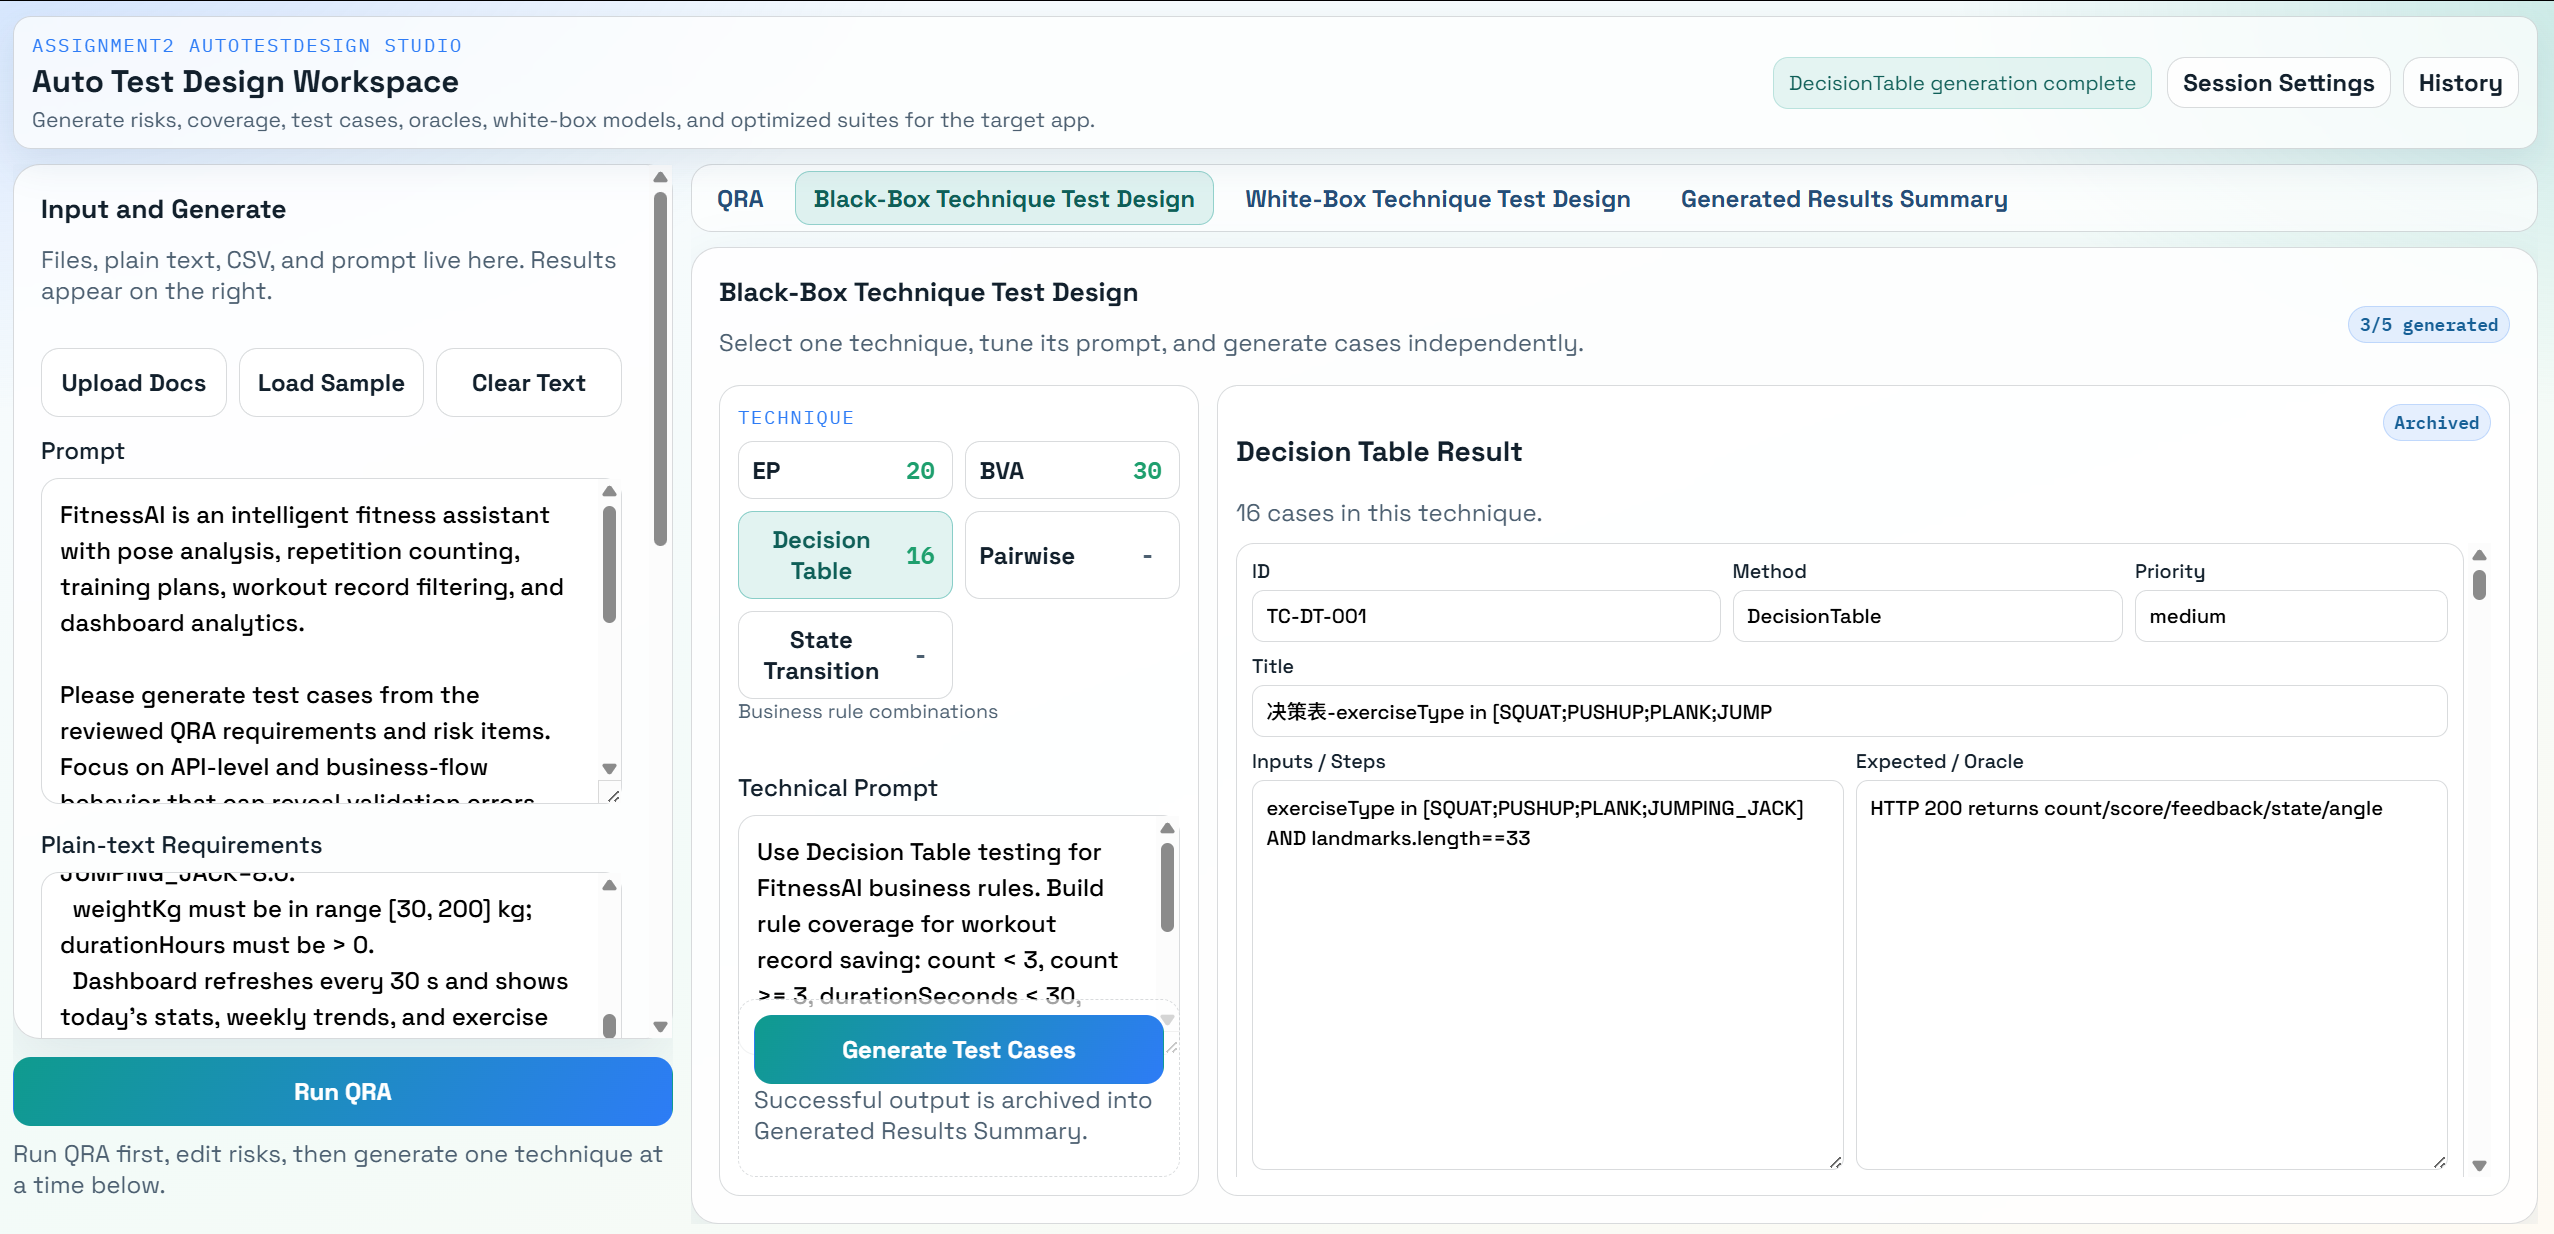
\includegraphics[width=0.9\textwidth]{contents/figure/fitnessai/Black_DT.png}
    \end{columns}
\end{frame}

\begin{frame}{Detailed Test Design: Pairwise}
    \begin{columns}[T]
        \column{0.42\textwidth}
        \scriptsize
        \begin{block}{Technique}
            \begin{itemize}
                \item Pairwise covers parameter pairs over \texttt{exerciseType}, \texttt{minScore}, and \texttt{sortBy}
            \end{itemize}
        \end{block}

        \begin{block}{Result}
            \begin{itemize}
                \item It contributes 6 cases and compresses the combination space
                \item The black-box layer totals 72 cases and remains reviewable in the tool
            \end{itemize}
        \end{block}

        \column{0.52\textwidth}
        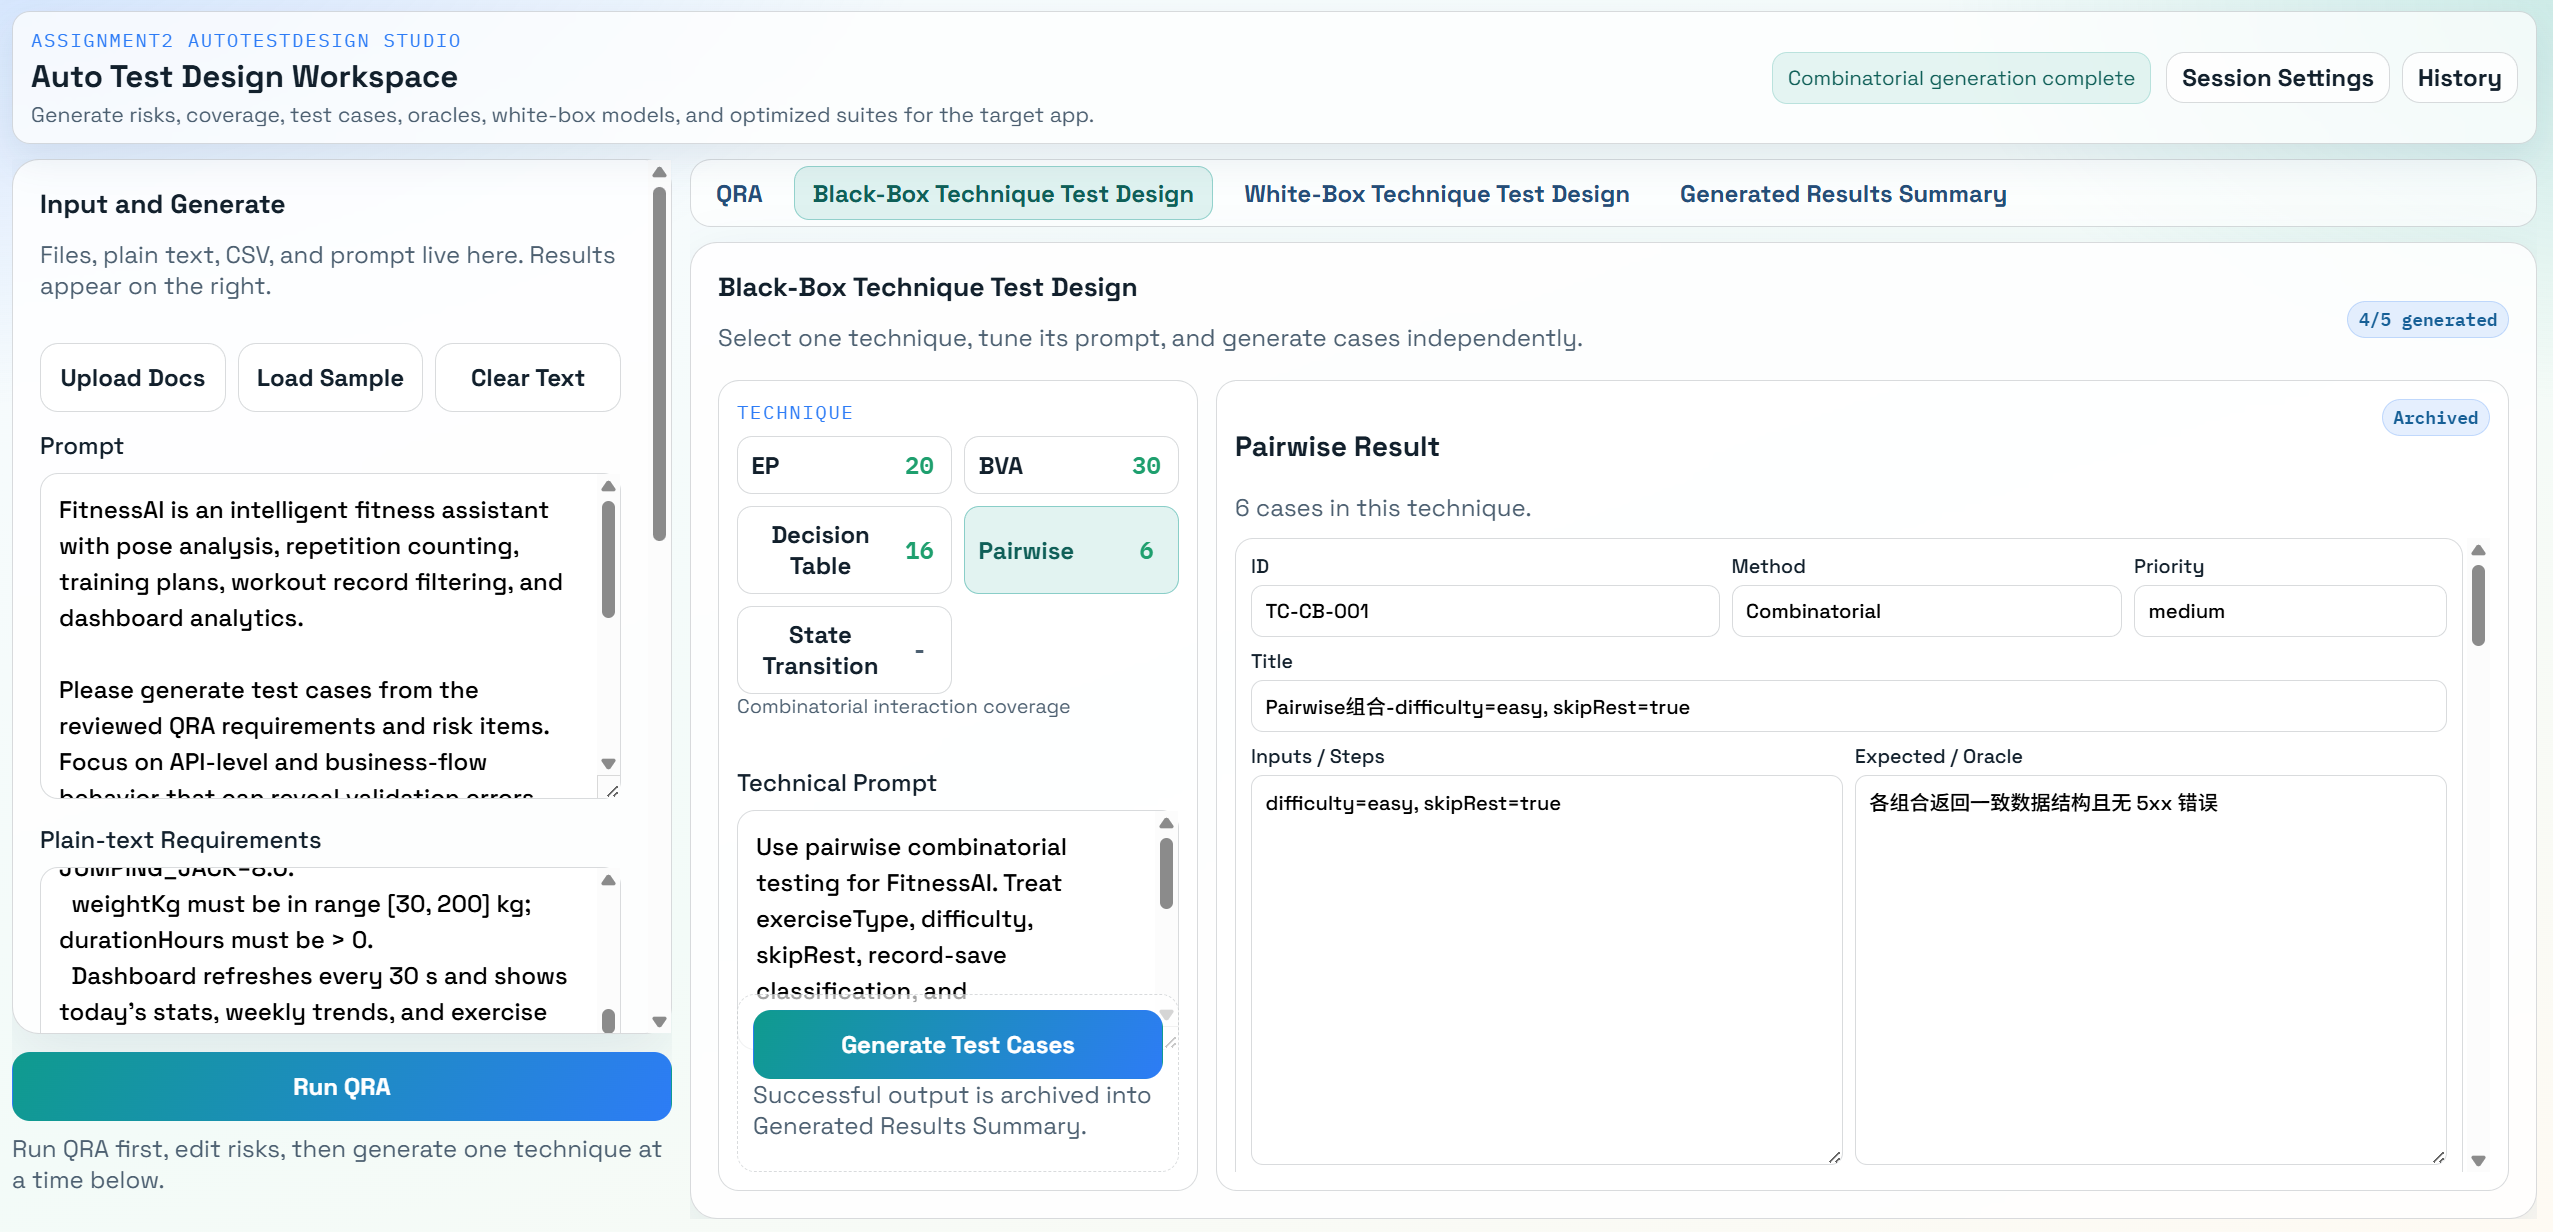
\includegraphics[width=0.9\textwidth]{contents/figure/fitnessai/Black_P.png}
    \end{columns}
\end{frame}

\begin{frame}{Design Example: Boundary Validation}
    \small
    \begin{block}{Landmark Boundary Review}
        \begin{itemize}
            \item The tool first treated \texttt{32/33/34} as symmetric boundaries
            \item Execution showed that \texttt{32} triggers \texttt{4xx}, while \texttt{34/35} still pass validation
            \item The real implementation is therefore not a strict ``exactly 33 landmarks only'' model
            \item This is a representative case where human review corrects AI-generated assumptions
        \end{itemize}
    \end{block}
\end{frame}

\begin{frame}{Design Example: Rules and Combinations}
    \small
    \begin{block}{Decision Table and Pairwise}
        \begin{itemize}
            \item The decision table covers all four truth combinations of \texttt{count < 3 \&\& duration < 30}
            \item Pairwise uses real history-filter parameters: \texttt{exerciseType}, \texttt{minScore}, and \texttt{sortBy}
            \item The generated cases stay close to the actual API instead of abstract variables
        \end{itemize}
    \end{block}
\end{frame}

\begin{frame}{State Transition and White-Box Testing}
    \begin{columns}[T]
        \column{0.32\textwidth}
        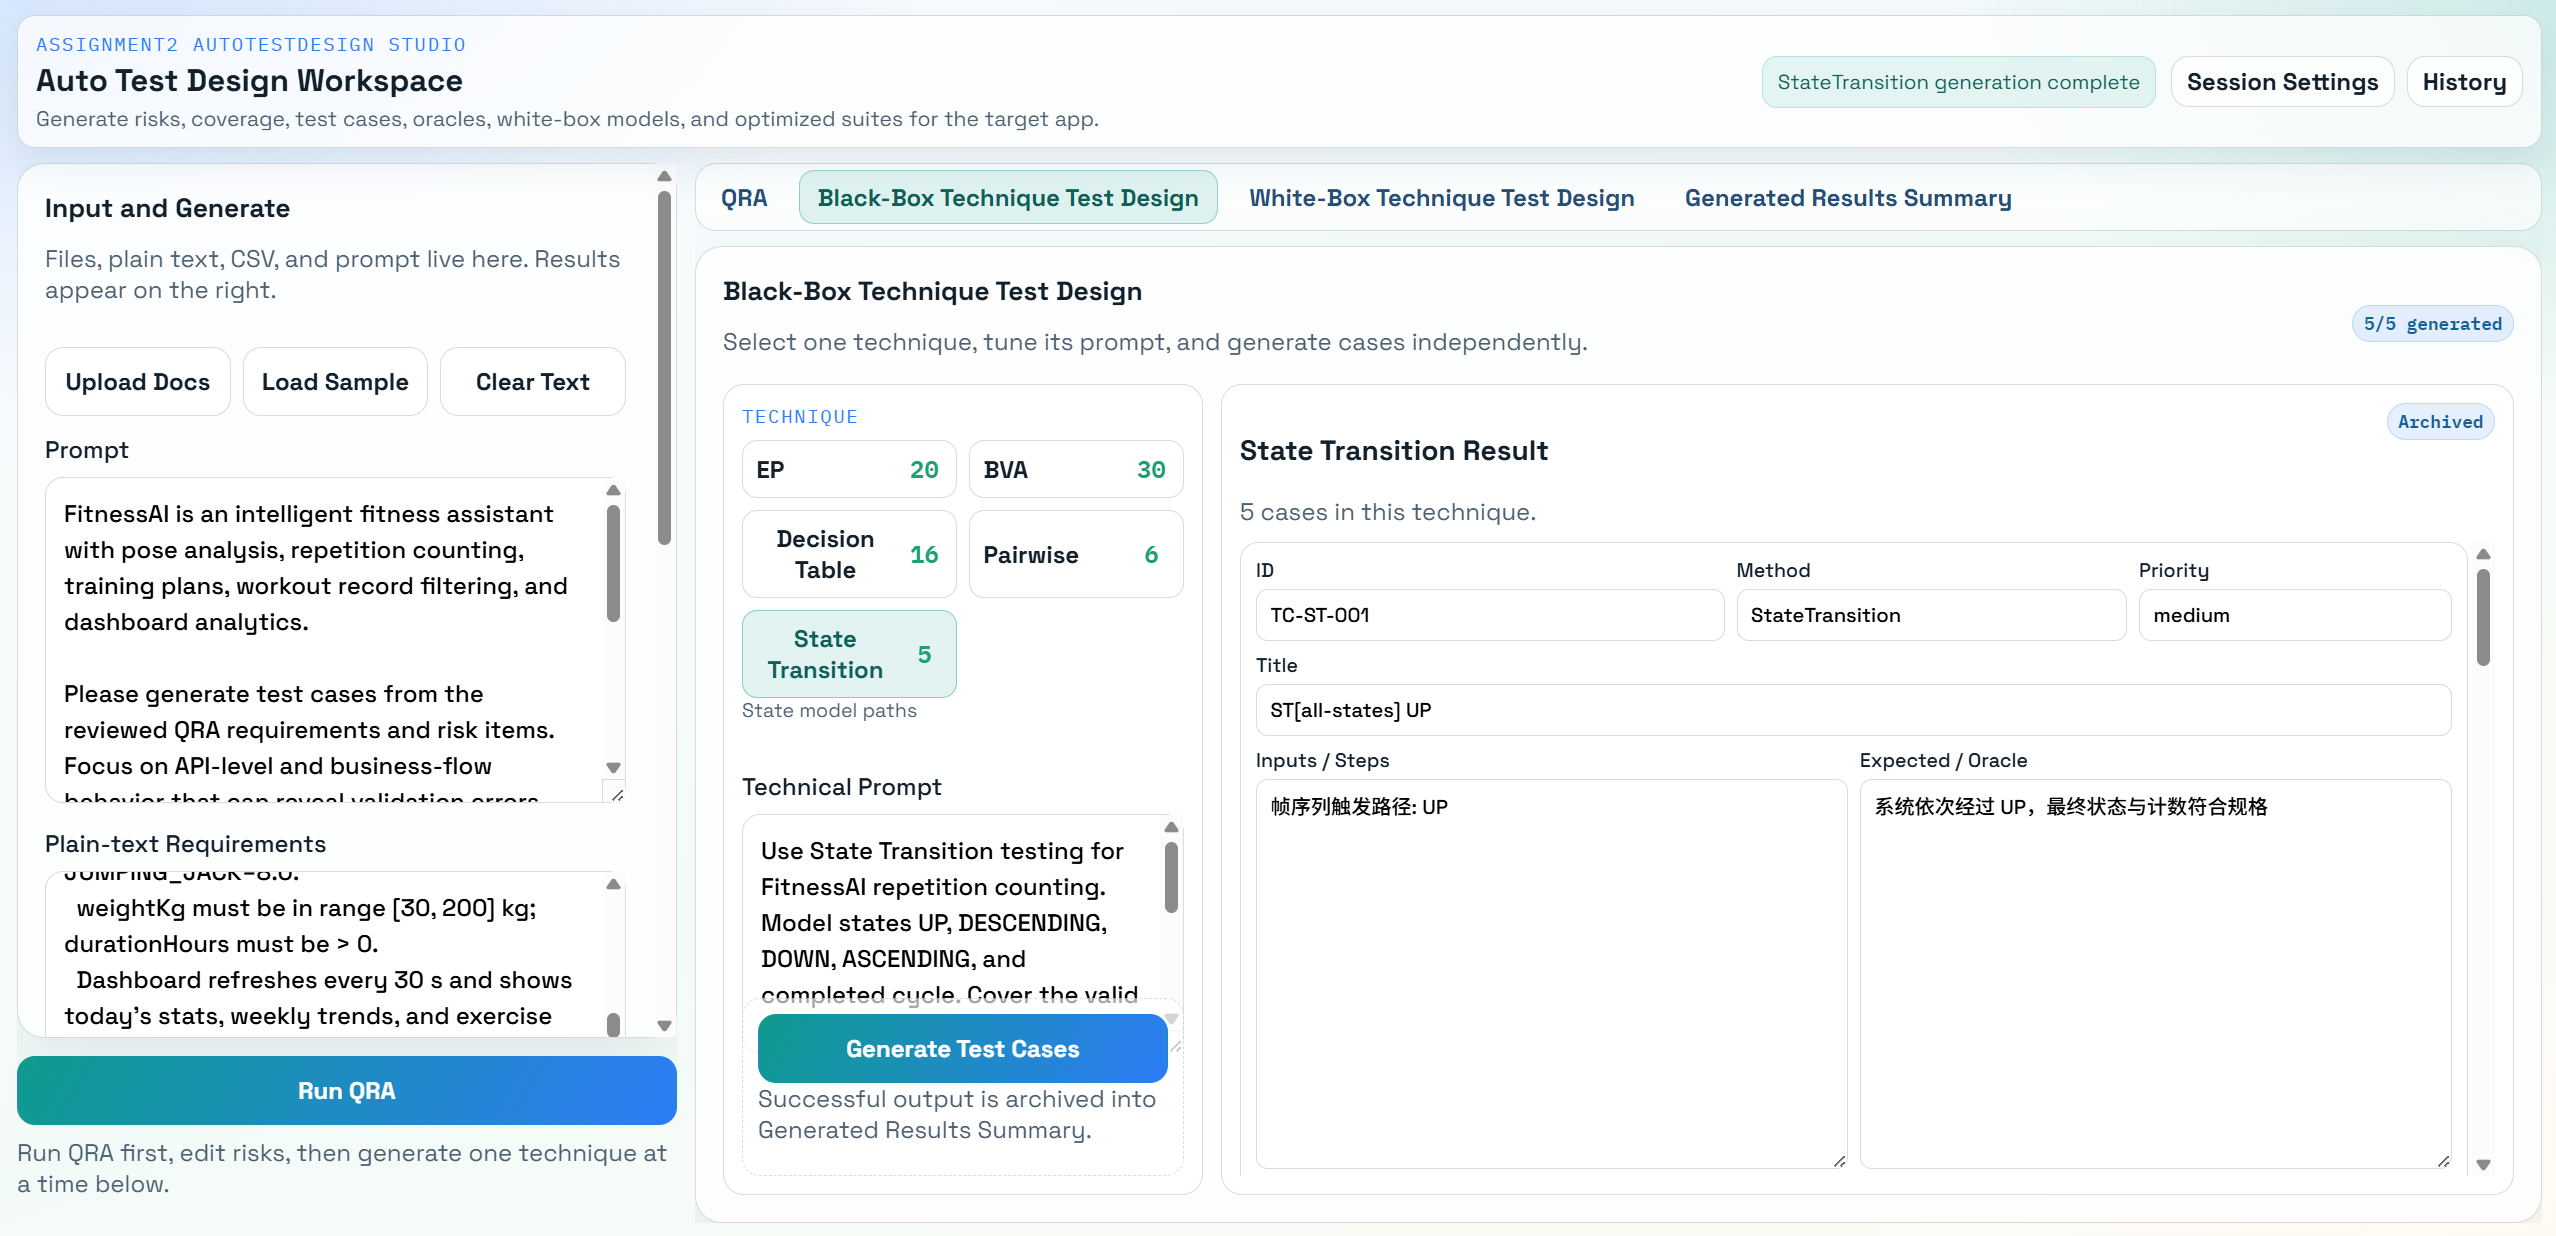
\includegraphics[width=\textwidth]{contents/figure/fitnessai/Black_ST.png}

        \column{0.32\textwidth}
        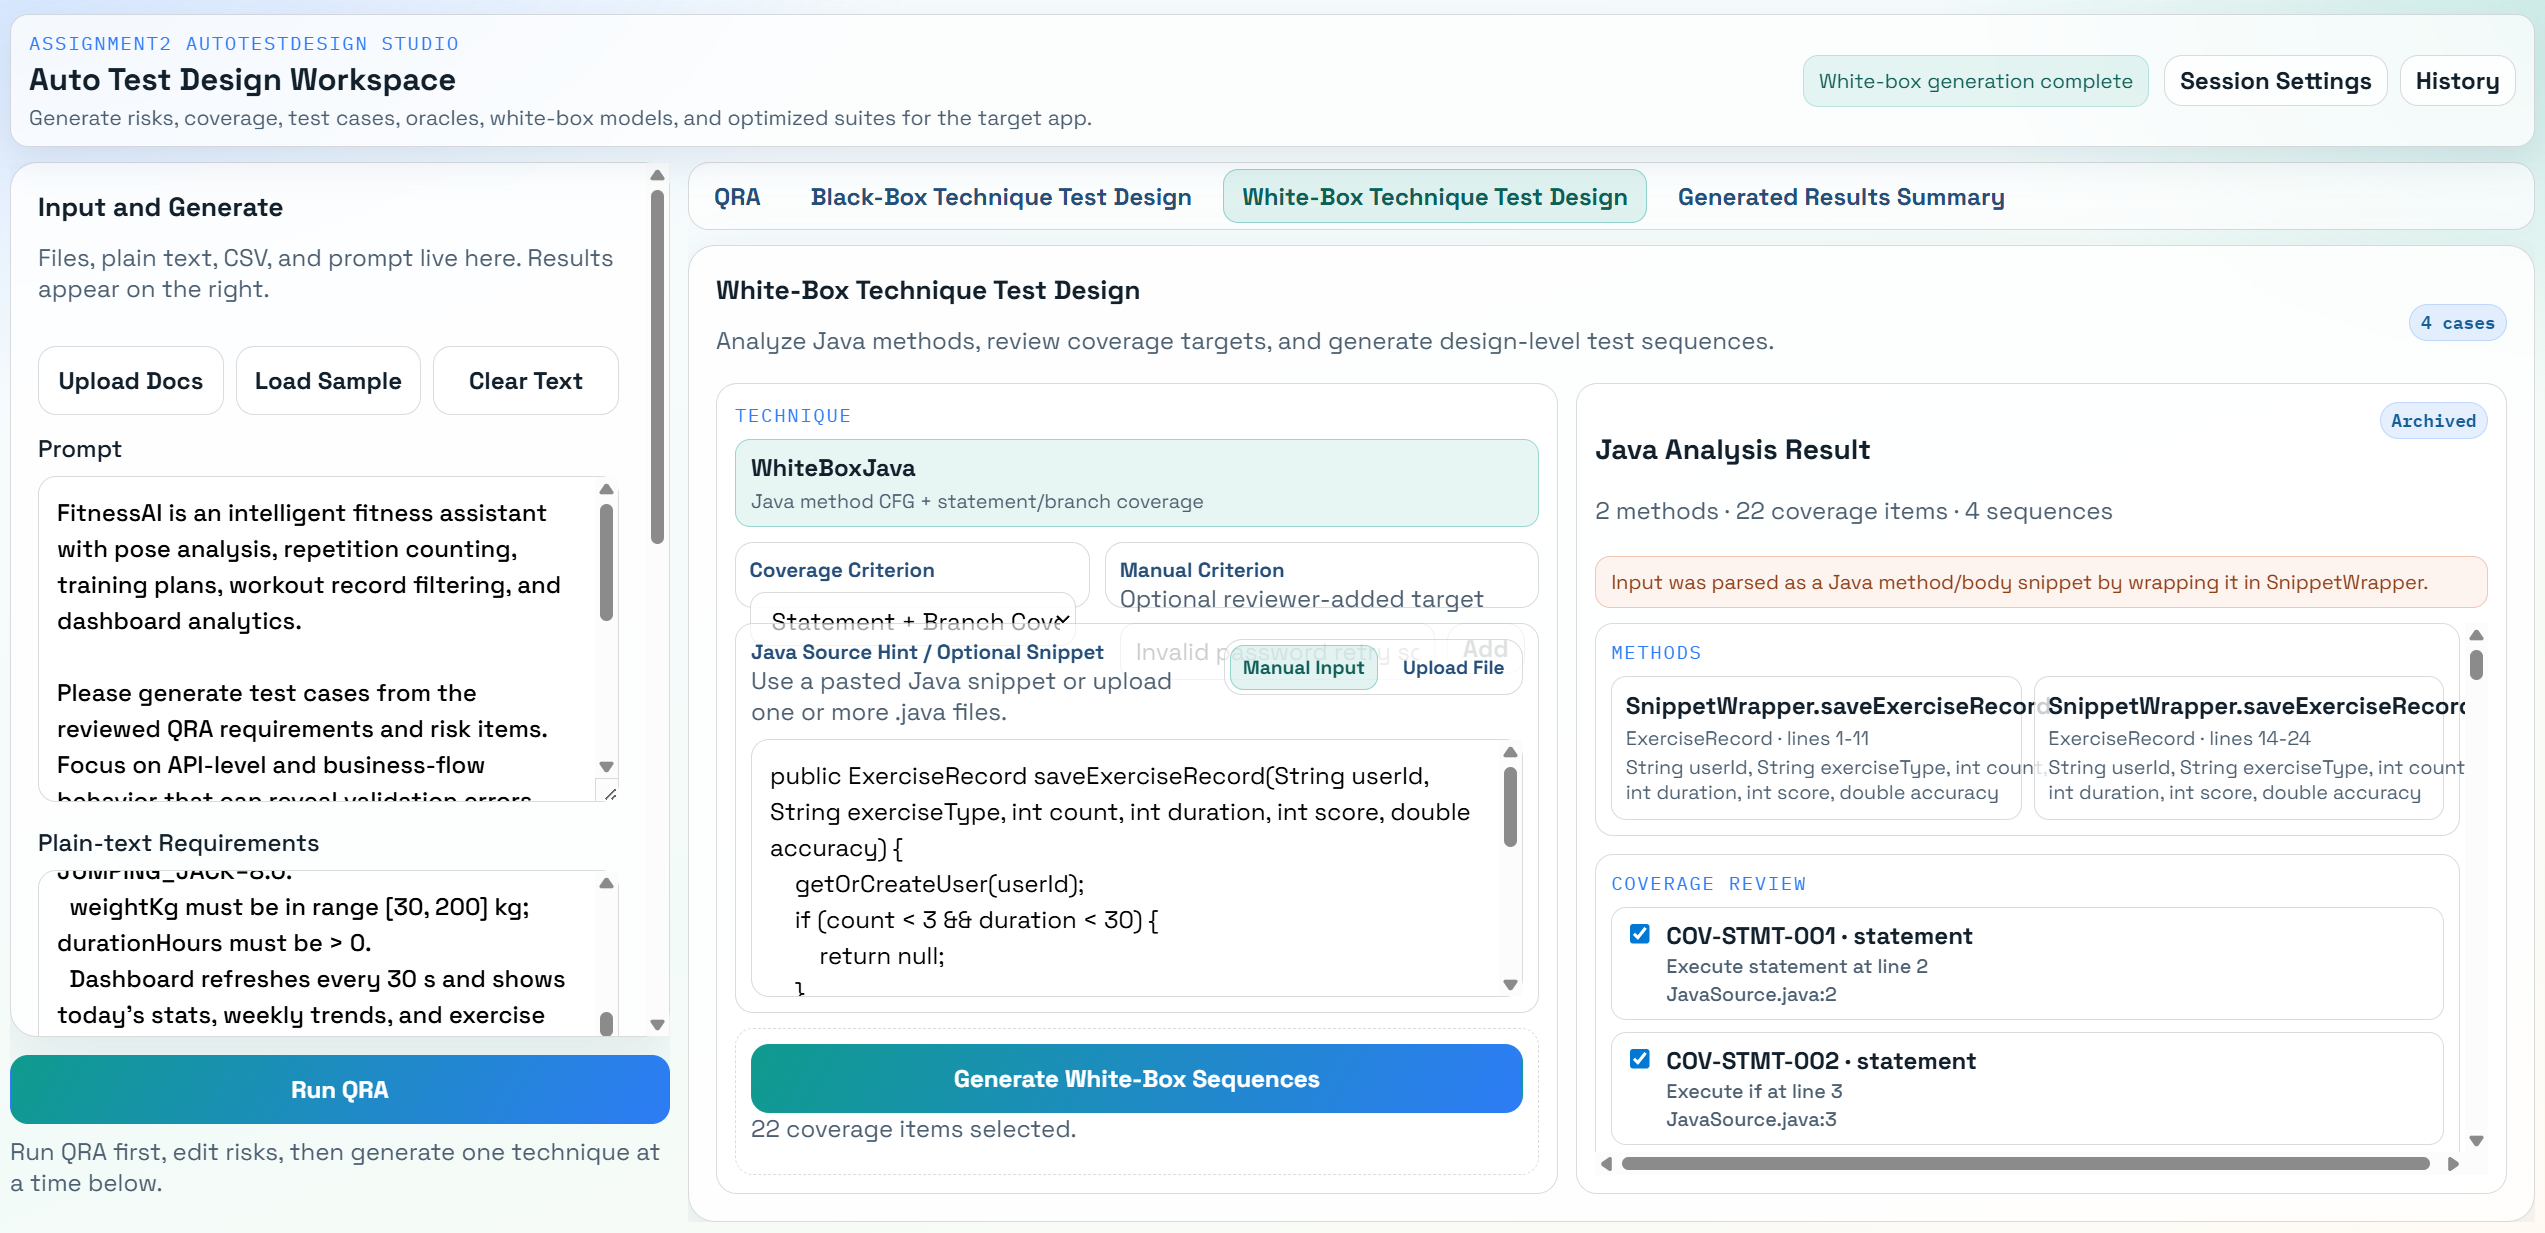
\includegraphics[width=\textwidth]{contents/figure/fitnessai/White_Coverage.png}

        \column{0.32\textwidth}
        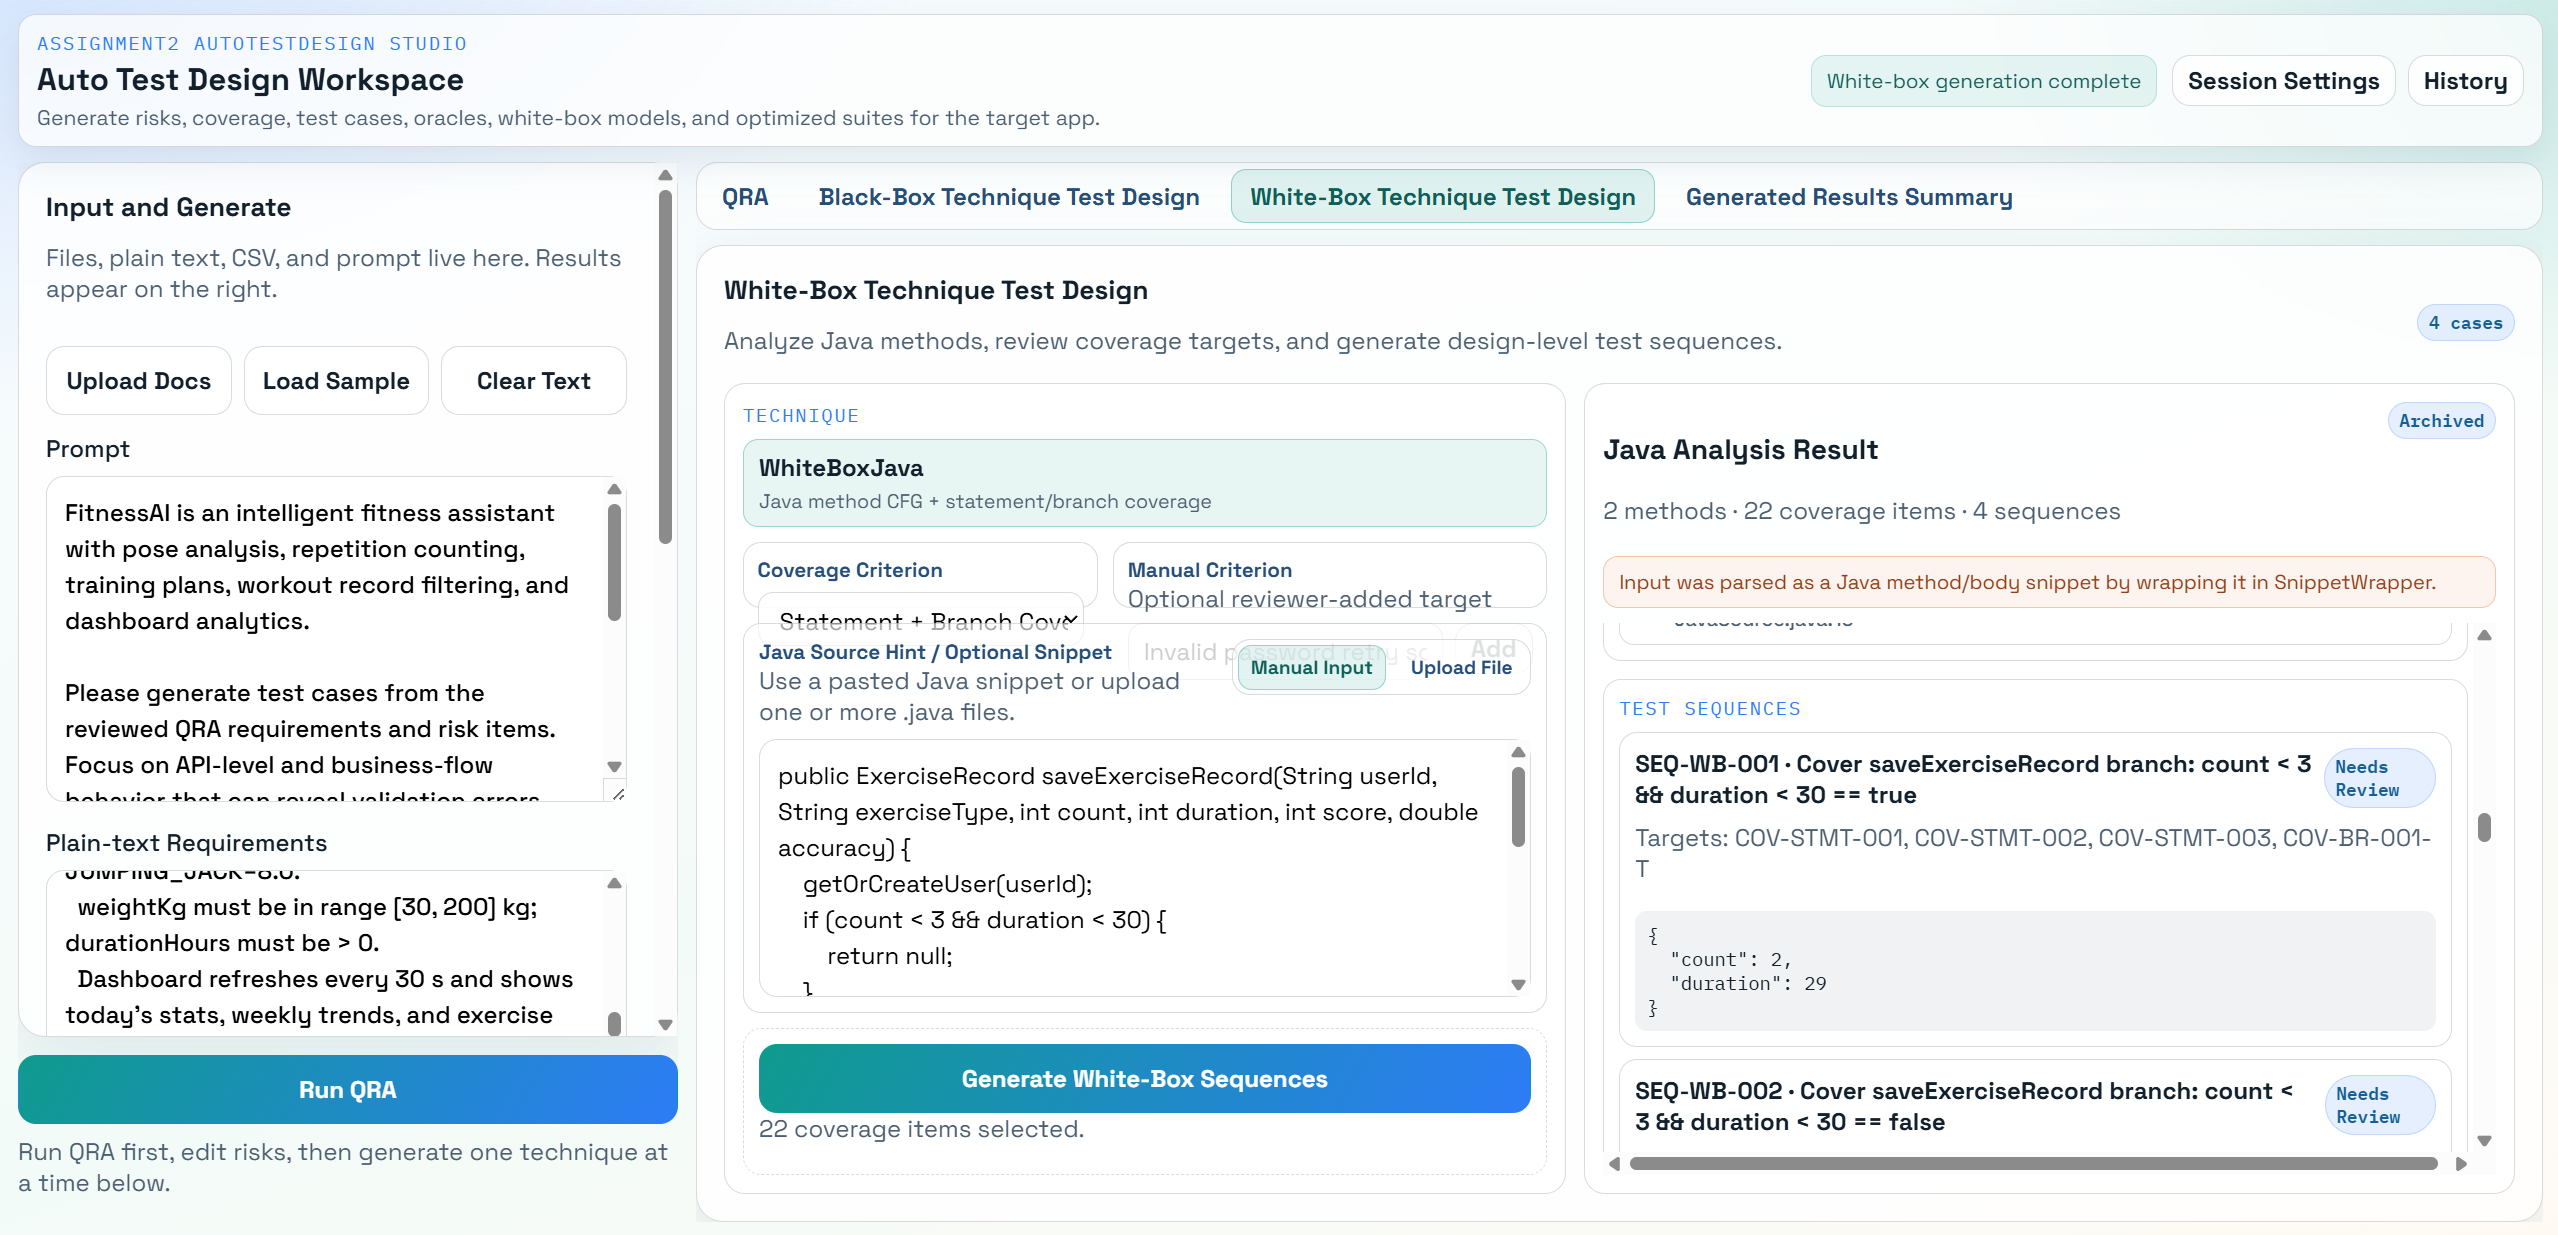
\includegraphics[width=\textwidth]{contents/figure/fitnessai/White_Sequence.png}
    \end{columns}

    \vspace{0.4em}
    \footnotesize
    \begin{itemize}
        \item State Transition: four primary states plus one reset scenario, for a total of five sequences
        \item WhiteBox Java: two method instances, 22 coverage items, and four sequences
        \item The target method is \texttt{saveExerciseRecord}, with the core branch \texttt{count < 3 \&\& duration < 30}
    \end{itemize}
\end{frame}

\begin{frame}{Automated Execution Results}
    \begin{columns}[T]
        \column{0.48\textwidth}
        \footnotesize
        \begin{block}{Execution Configuration}
            \begin{itemize}
                \item Test framework: JUnit 5 + MockMvc
                \item Data isolation: \texttt{@Transactional}
                \item Reporting: Allure + \texttt{TestResultExtension}
            \end{itemize}
        \end{block}

        \begin{block}{Execution Results}
            \begin{itemize}
                \item Total test cases: 81
                \item Passed: 81
                \item Failed / errored / skipped: 0 / 0 / 0
                \item Success rate: 100\%
            \end{itemize}
        \end{block}

        \column{0.46\textwidth}
        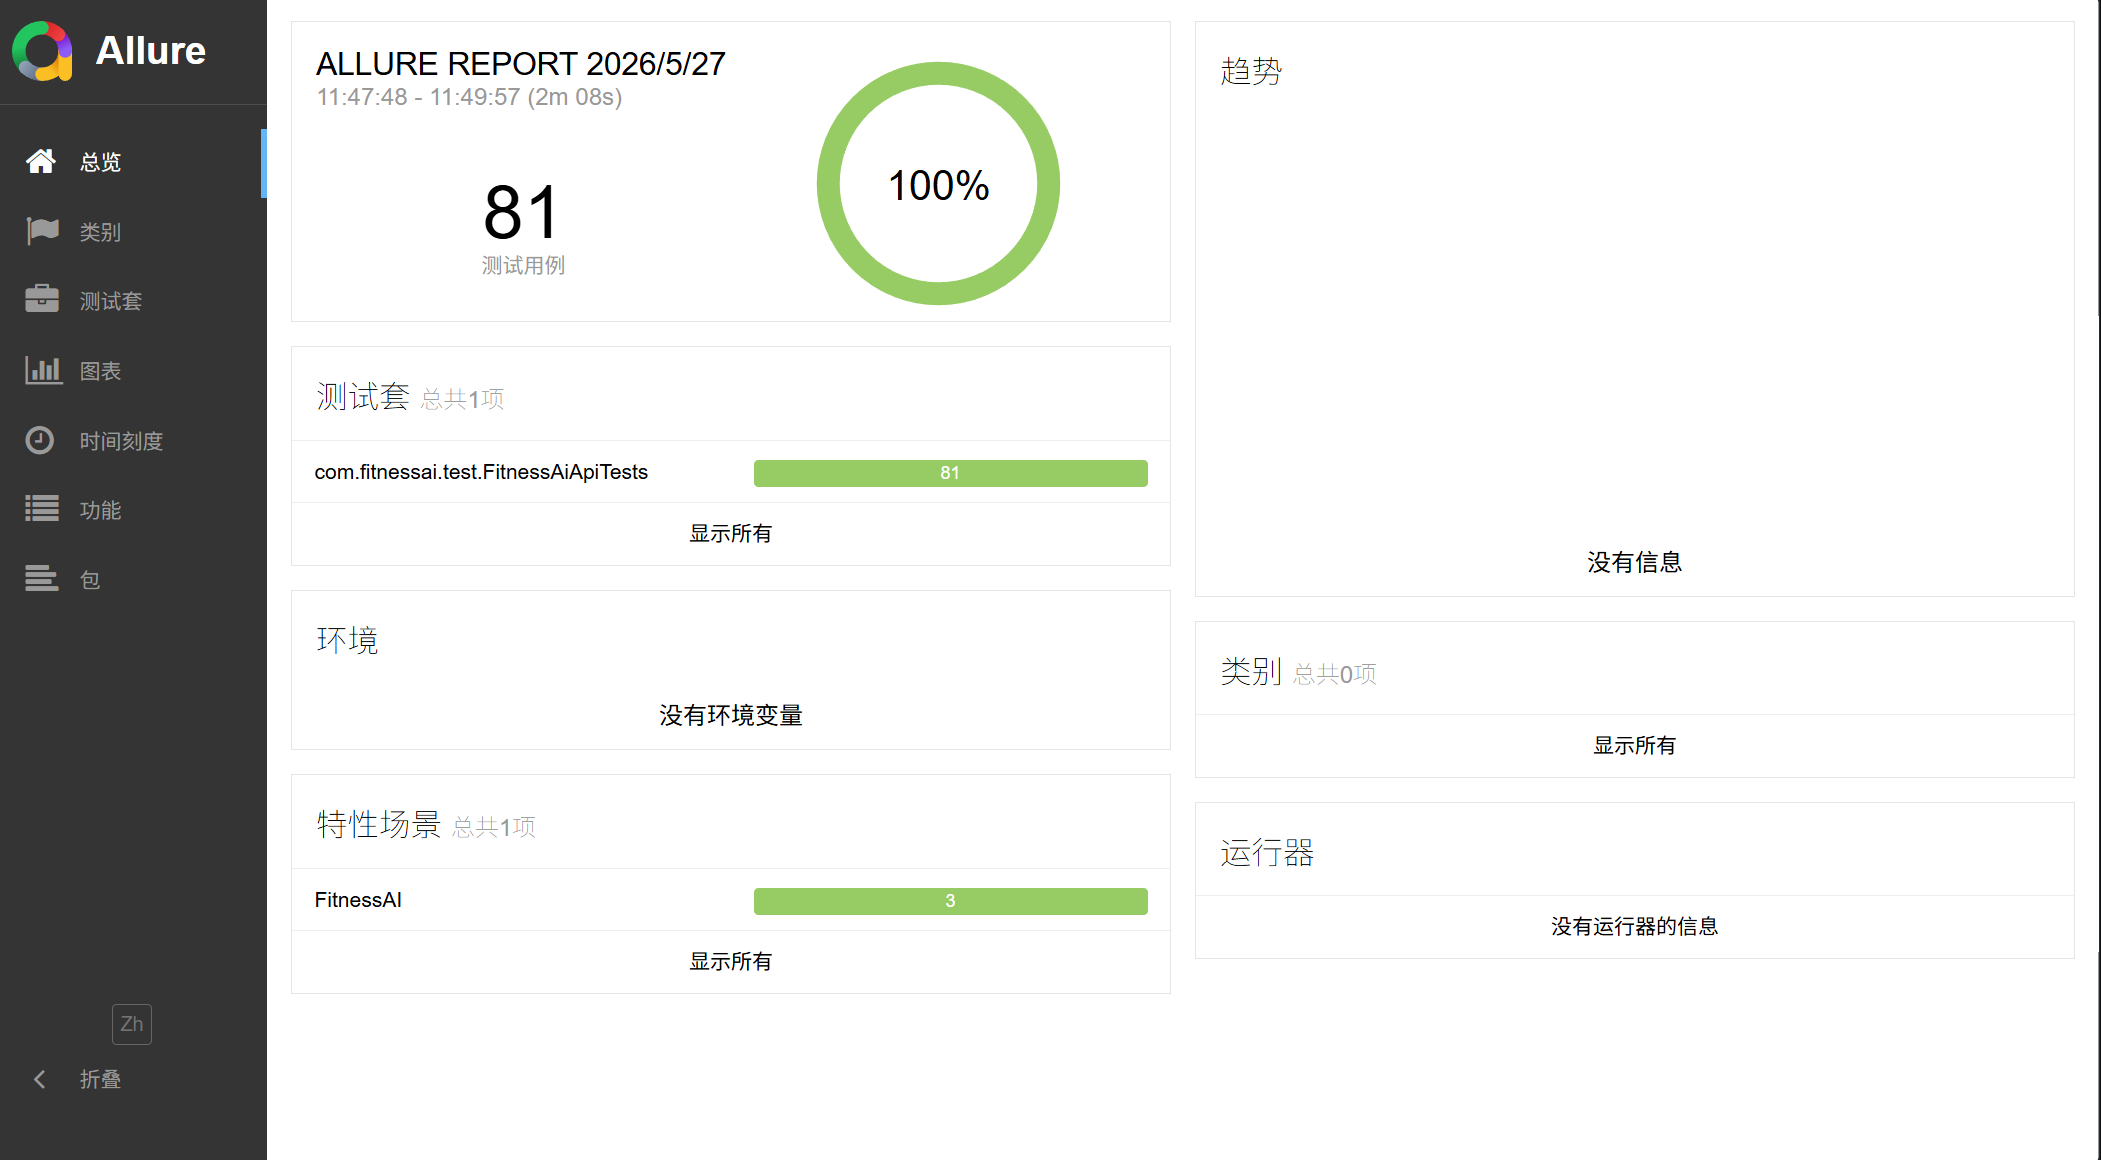
\includegraphics[width=0.92\textwidth]{contents/figure/fitnessai/allure-report-1.png}
    \end{columns}
\end{frame}

\begin{frame}{Allure Report Views}
    \begin{columns}[T]
        \column{0.49\textwidth}
        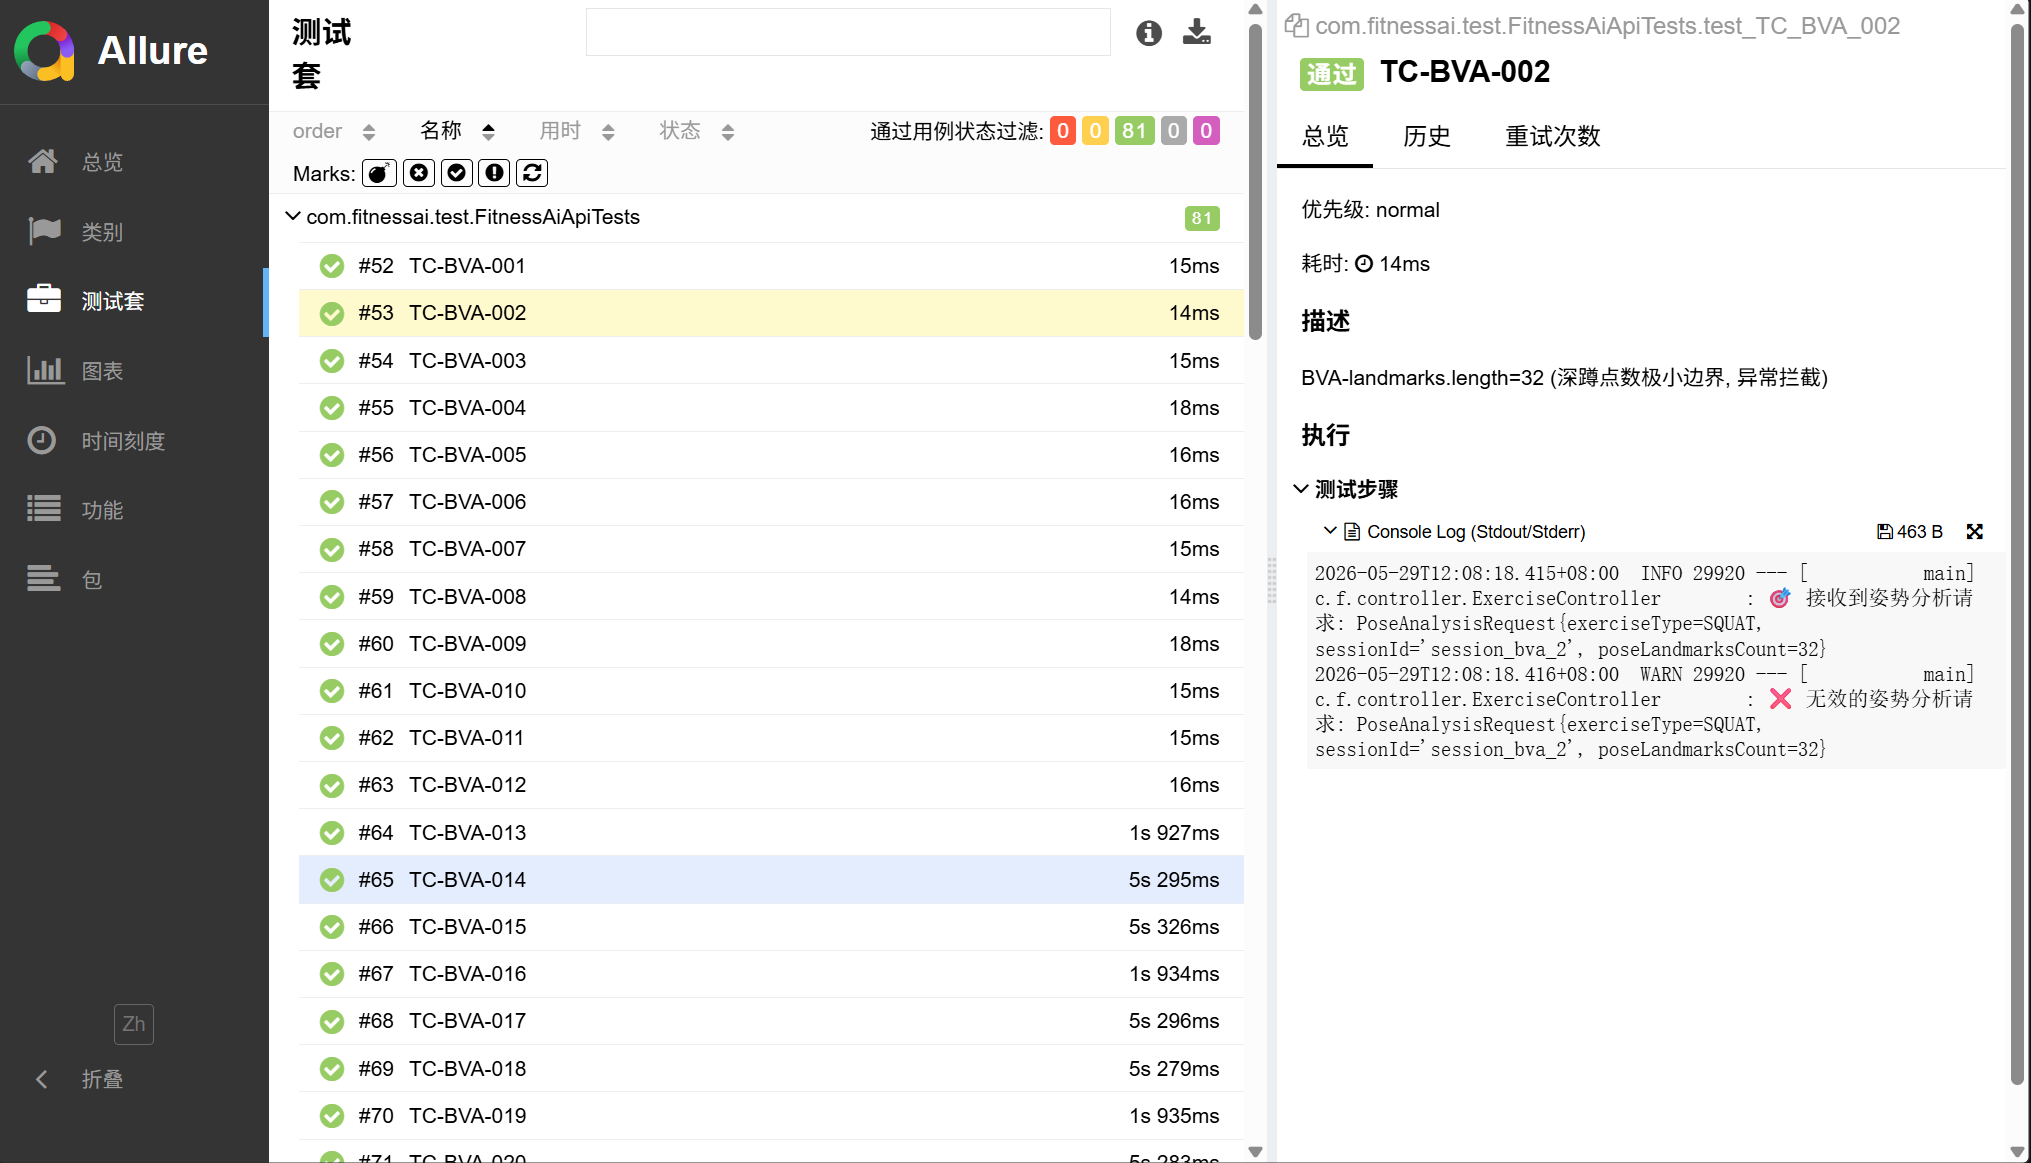
\includegraphics[width=\textwidth]{contents/figure/fitnessai/allure-report-2.png}

        \column{0.49\textwidth}
        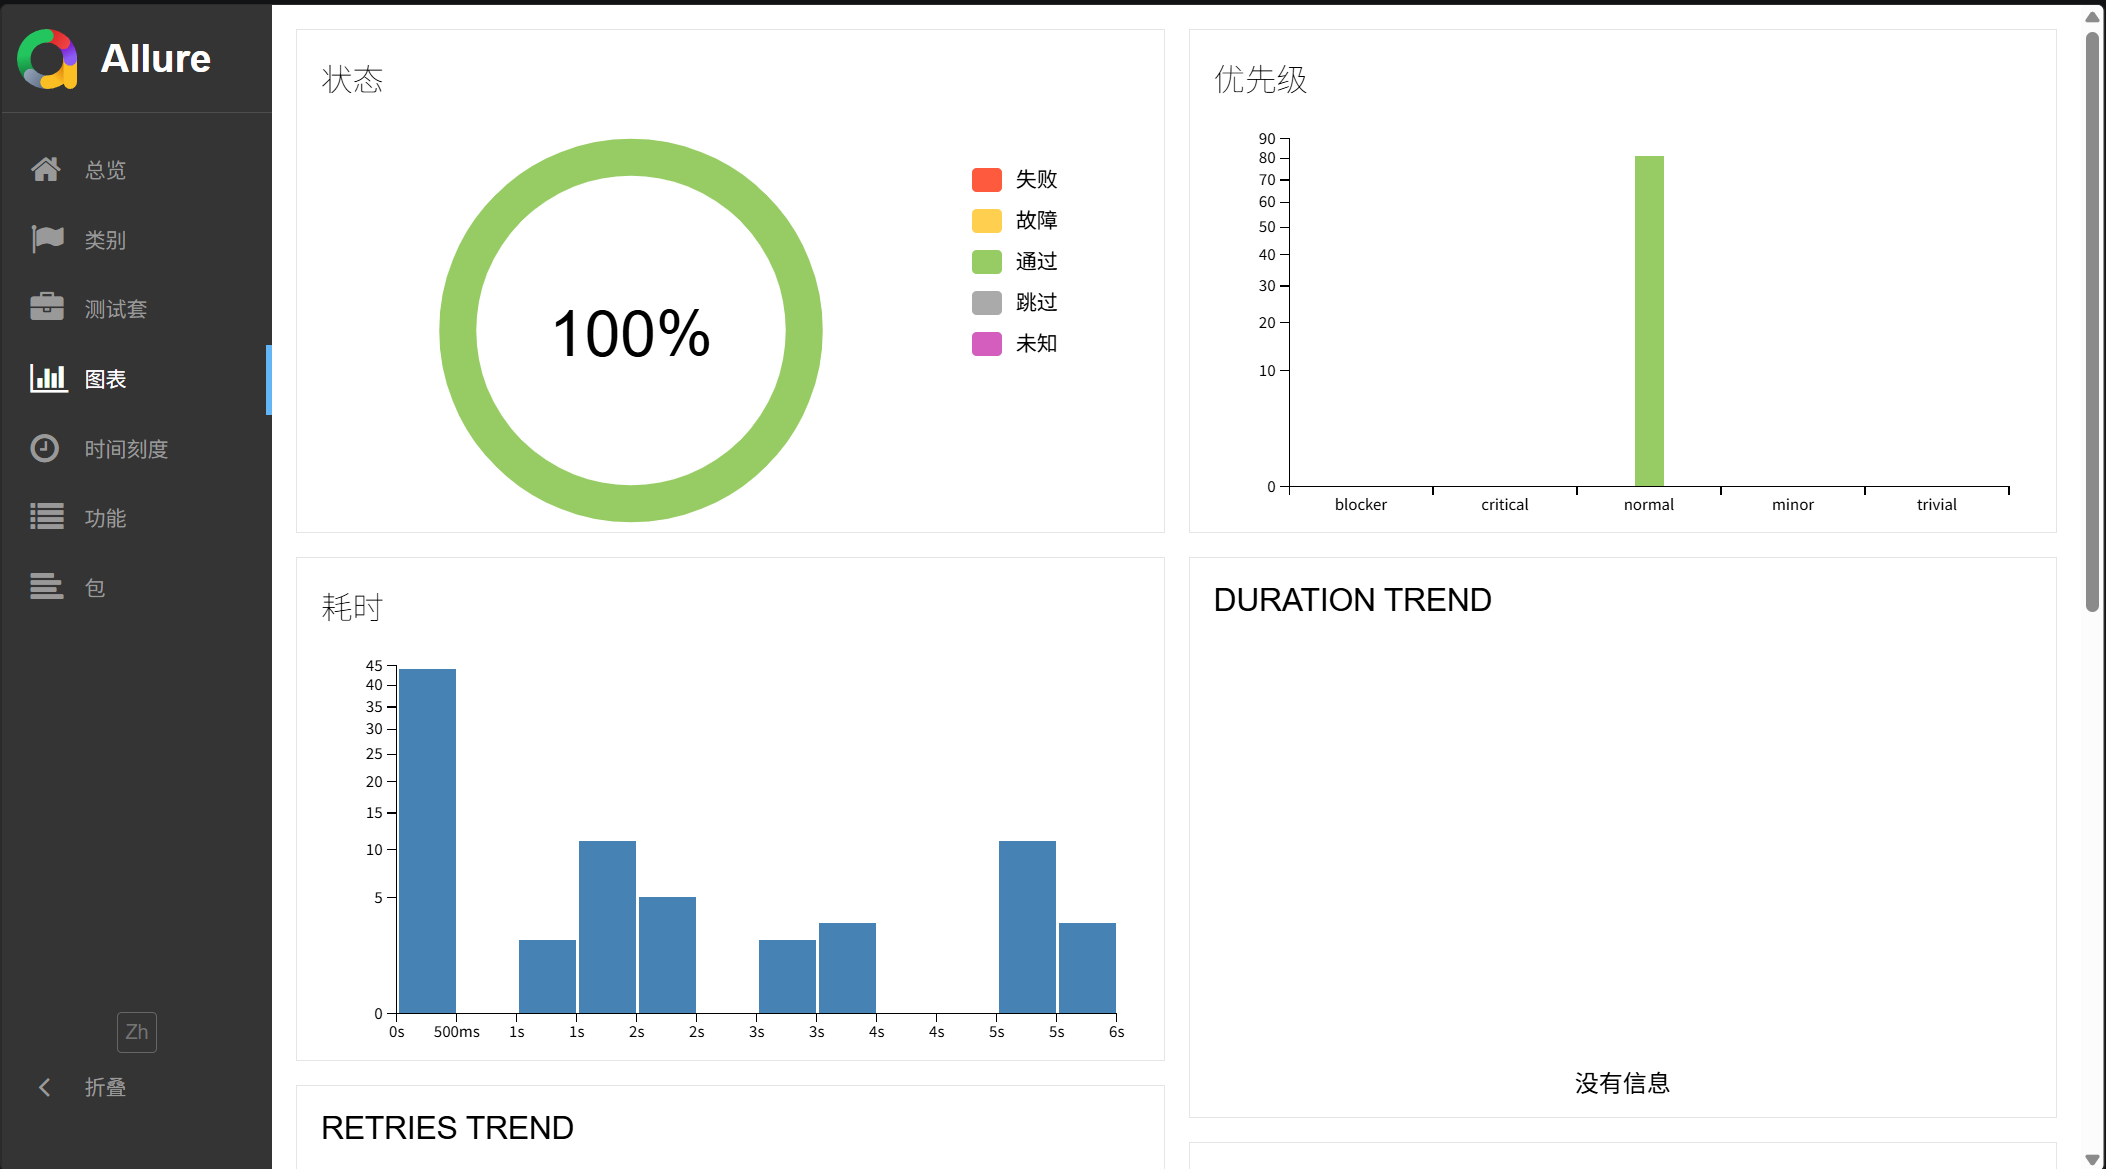
\includegraphics[width=\textwidth]{contents/figure/fitnessai/allure-report-3.png}
    \end{columns}

    \vspace{0.5em}
    \footnotesize
    The left image shows the suite and categorization view, while the right image shows execution charts. Together, they support the conclusion that all 81 test cases passed.
\end{frame}

\begin{frame}{Coverage Results}
    \begin{columns}[T]
        \column{0.52\textwidth}
        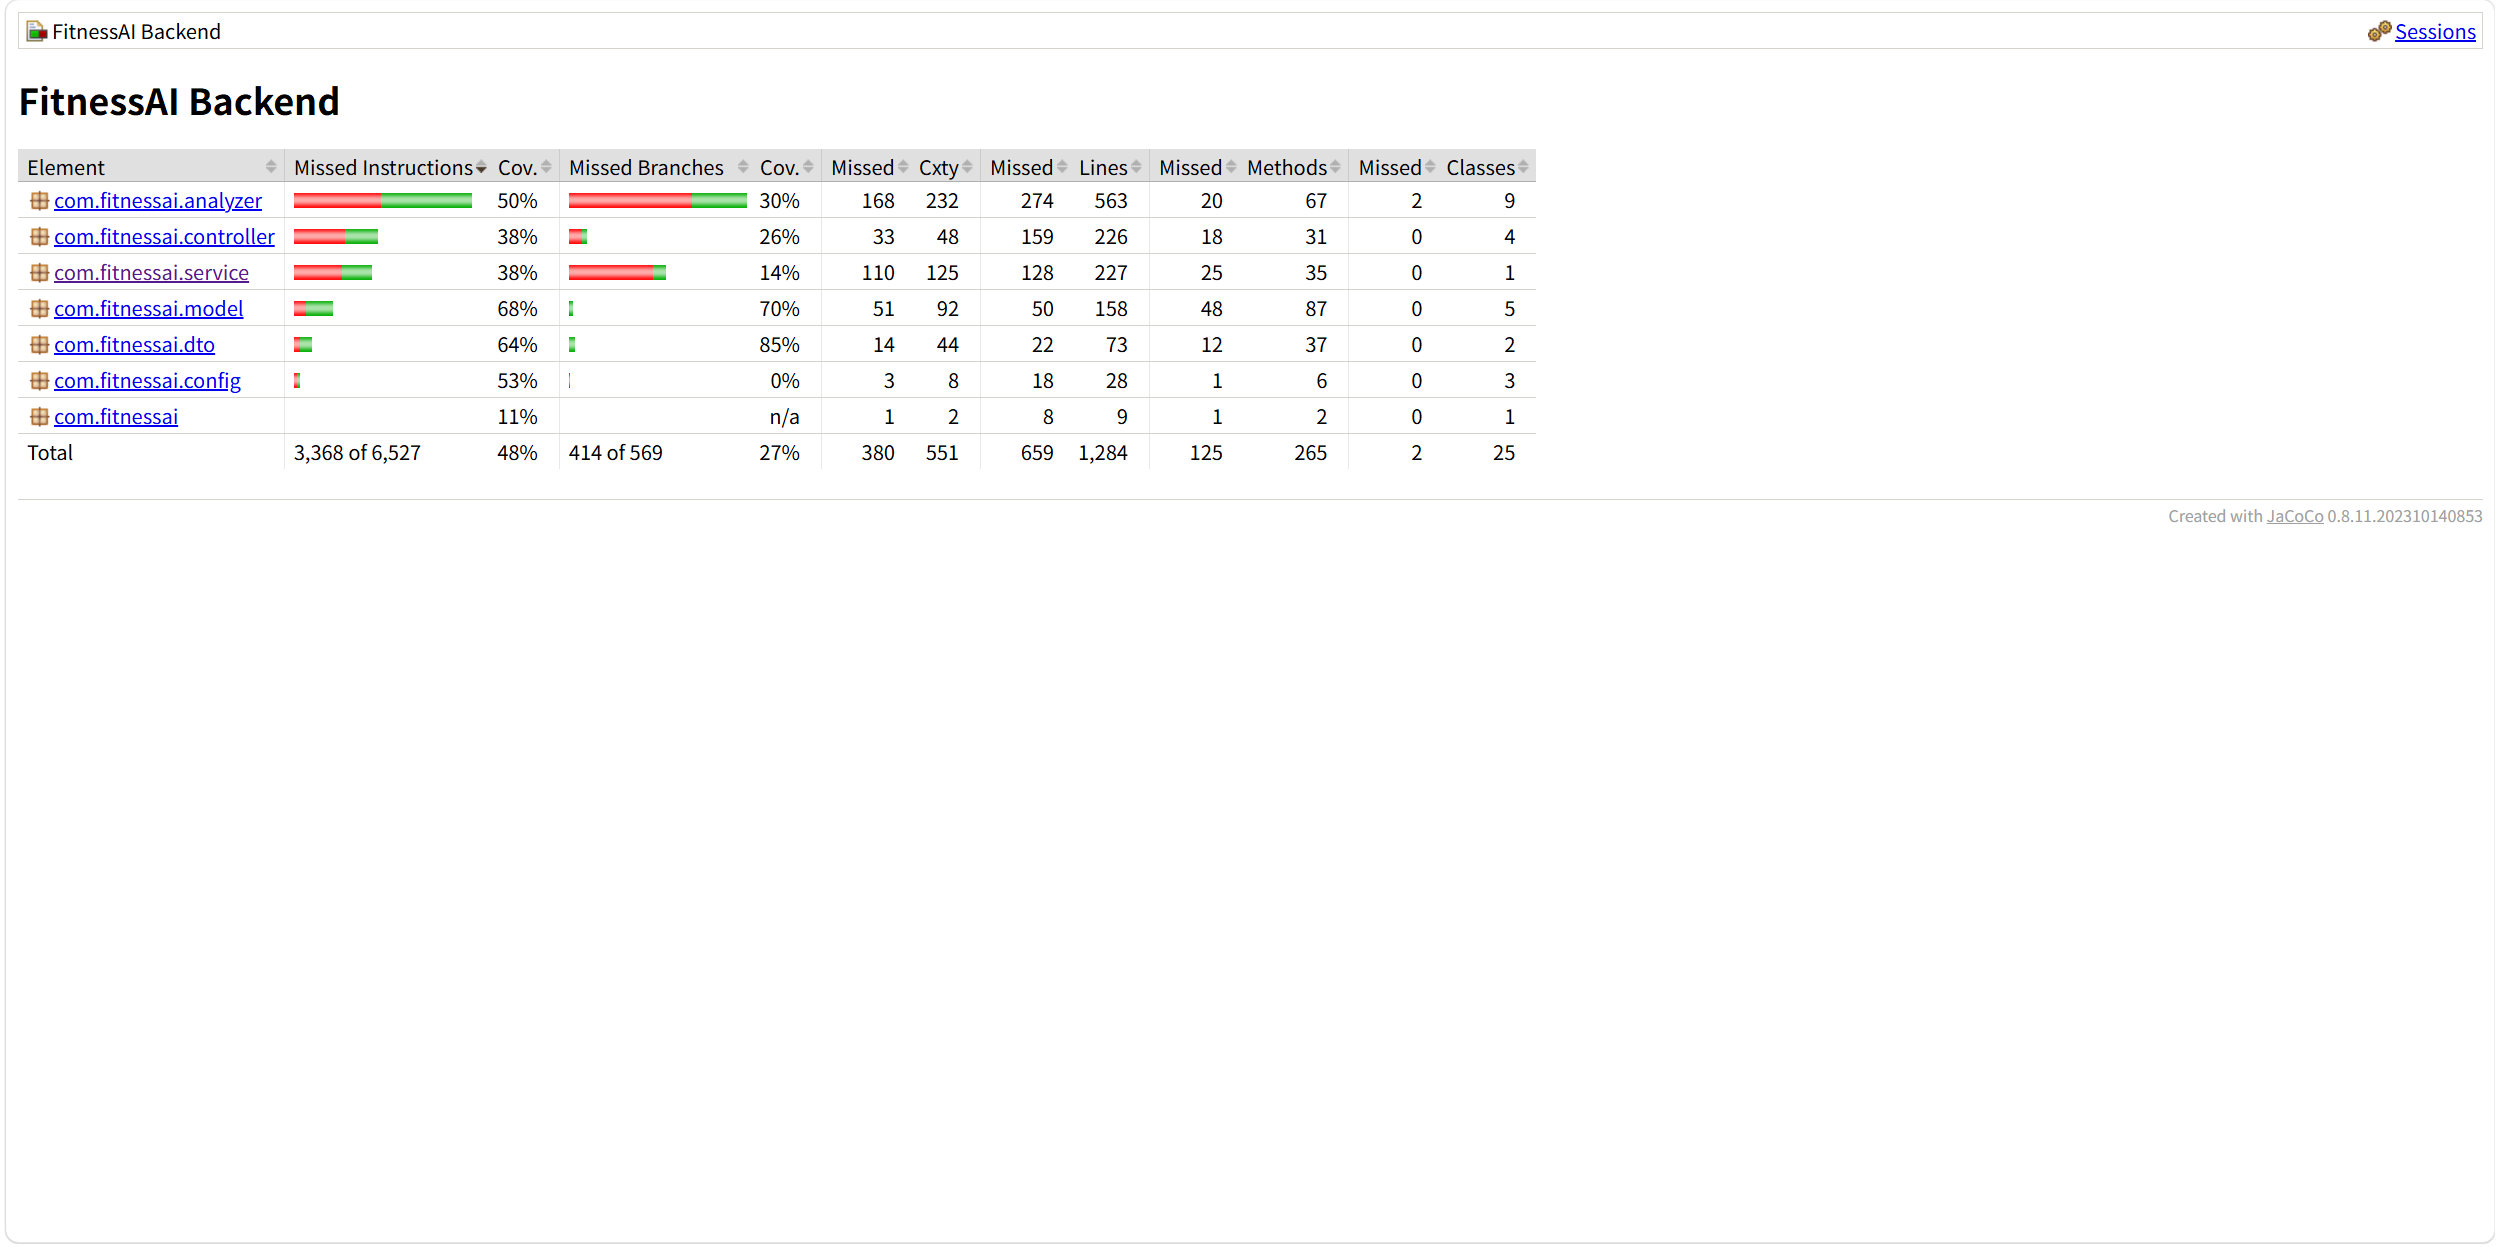
\includegraphics[width=\textwidth]{contents/figure/fitnessai/Jacoco-1.png}

        \column{0.42\textwidth}
        \scriptsize
        \begin{tabular}{@{}lc@{}}
            \toprule
            \textbf{Target} & \textbf{Coverage} \\ \midrule
            \texttt{saveExerciseRecord} & 100/100 \\
            \texttt{SquatAnalyzer} & 92.8 / 80.0 \\
            \texttt{ExerciseController} & 48.1 / 66.7 \\
            \bottomrule
        \end{tabular}
    \end{columns}

    \vspace{0.5em}
    \footnotesize
    The evidence shows full coverage on the key persistence method and useful branch coverage on the pose-analysis path.
\end{frame}

\begin{frame}{Evidence-Based Corrections}
    \small
    \begin{block}{Corrections Found During Execution}
        \begin{itemize}
            \item \texttt{TC-BVA-002}: 32 landmarks are invalid and lead to \texttt{4xx}
            \item \texttt{TC-ST-005}: the implemented check is the reset endpoint, not a narrative-level COOLDOWN state
            \item \texttt{TC-EP-017} / \texttt{TC-DT-015}: the third \texttt{difficulty} item is currently \texttt{medium}
        \end{itemize}
    \end{block}

    \begin{block}{Conclusion}
        \begin{itemize}
            \item The tool is responsible for high-coverage generation
            \item Human review is responsible for final semantic alignment
            \item Execution evidence closes the loop between design and implementation
        \end{itemize}
    \end{block}
\end{frame}

\begin{frame}{Tool Value and Limitations}
    \small
    \begin{columns}[T]
        \column{0.48\textwidth}
        \begin{block}{Tool Value}
            \begin{itemize}
                \item Connects requirements, risks, coverage items, test cases, and execution evidence
                \item Supports interactive review instead of blindly accepting AI output
                \item Is especially effective for API-centric systems with explicit business rules
            \end{itemize}
        \end{block}

        \column{0.48\textwidth}
        \begin{block}{Current Limitations}
            \begin{itemize}
                \item UI-layer behavior and browser-level behavior were not the focus of this round
                \item Security and performance testing are still supplementary rather than exhaustive
                \item Some semantics still require human correction based on code and execution evidence
            \end{itemize}
        \end{block}
    \end{columns}

    \vspace{0.5em}
    \footnotesize
    Therefore, the project ultimately adopts a three-stage validation strategy: tool generation + human review + automated execution evidence.
\end{frame}

%% summary.tex
%% Copyright 2023 TJ-CSCCG
%
% This work may be distributed and/or modified under the
% conditions of the LaTeX Project Public License, either version 1.3
% of this license or (at your option) any later version.
% The latest version of this license is in
%   http://www.latex-project.org/lppl.txt
% and version 1.3 or later is part of all distributions of LaTeX
% version 2003/12/01 or later.
%
% This work has the LPPL maintenance status "maintained".
%
% This Current Maintainer of this work is Rizhong Lin.
%
% This work consists of all the *.tex and *.sty files in
%   https://github.com/TJ-CSCCG/Tongji-Beamer
\section{总结}

\begin{frame}{总结}
    \footnotesize
    \begin{block}{项目产出}
        \begin{itemize}
            \item 实现了一个可运行的 AutoTestDesign 工具，并将其应用到 FitnessAI
            \item 形成了从风险分析到自动化执行的完整测试闭环
            \item 输出了可审查、可执行、可追溯的测试工件与证据
        \end{itemize}
    \end{block}

    \begin{block}{关键结论}
        \begin{itemize}
            \item 生成结果：10 条需求、37 个覆盖项、81 条用例、6 种设计方法
            \item 人机协同：交互审查修正 AI 偏差，最终 81/81 自动化测试全部通过
            \item 证据链：QRA、Summary、Allure、JaCoCo 均已落地
        \end{itemize}
    \end{block}
\end{frame}

\begin{frame}
    \begin{center}
        \Huge\bfseries Thank You
    \end{center}
\end{frame}


\end{document}
